%  LaTeX support: latex@mdpi.com 


%=================================================================
\documentclass[fire,article,submit,pdftex,moreauthors]{Definitions/mdpi} 


%=================================================================
% MDPI internal commands - do not modify
\firstpage{1} 
\makeatletter 
\setcounter{page}{\@firstpage} 
\makeatother
\pubvolume{1}
\issuenum{1}
\articlenumber{0}
\pubyear{2025}
\copyrightyear{2025}
%\externaleditor{Firstname Lastname} % More than 1 editor, please add `` and '' before the last editor name
\datereceived{ } 
% \daterevised{ } % Comment out if no revised date
\dateaccepted{ } 
\datepublished{ } 
%\datecorrected{} % For corrected papers: "Corrected: XXX" date in the original paper.
%\dateretracted{} % For retracted papers: "Retracted: XXX" date in the original paper.
\hreflink{https://doi.org/} % If needed use \linebreak
%\doinum{}
%\pdfoutput=1 % Uncommented for upload to arXiv.org
%\CorrStatement{yes}  % For updates
%\longauthorlist{yes} % For many authors that exceed the left citation part
\tolerance=5000  % tolerate sparser lines, avoid divided words
\pretolerance=5000

%=================================================================
% Please use the following mathematics environments: Theorem, Lemma, Corollary, Proposition, Characterization, Property, Problem, Example, ExamplesandDefinitions, Hypothesis, Remark, Definition, Notation, Assumption
%% For proofs, please use the proof environment (the amsthm package is loaded by the MDPI class).

%=================================================================
% Full title of the paper (Capitalized)
\Title{A Recurrent Neural Network for Forecasting Fuel Moisture Content with Inputs from Numerical Weather Models}

% MDPI internal command: Title for citation in the left column
\TitleCitation{A Recurrent Neural Network for Forecasting Fuel Moisture Content with Inputs from Numerical Weather Models}


% Authors, for the paper (add full first names)
\Author{Jonathon Hirschi $^{1, *}$, Jan Mandel $^{1}$, Kyle Hilburn$^{2}$, Angel Farguell Caus $^{3}$}

%\longauthorlist{yes}

% MDPI internal command: Authors, for metadata in PDF
\AuthorNames{Jonathon Hirschi, Jan Mandel, Kyle Hilburn, Angel Farguell Caus}

% MDPI internal command: Authors, for citation in the left column, only choose below one of them according to the journal style


% Affiliations / Addresses (Add [1] after \address if there is only one affiliation.)
\address{%
$^{1}$ \quad Department of Mathematical and Statistical Sciences,
University of Colorado Denver, 1201 Larimer St.,
Denver, CO 80204, USA\\
$^{2}$ \quad Cooperative Institute for Research in the Atmosphere (CIRA), Colorado State University,
934 W Mountain Ave Fort Collins, CO 80521, USA\\
$^{3}$ \quad Wildfire Interdisciplinary Research Center, 
San Jose State University, 801 Duncan Hall,
One Washington Square,
San Jose, CA 95192-0126, USA}

% Contact information of the corresponding author
\corres{Correspondence: jonathon.hirschi@ucdenver.edu}

% Abstract 200 words max, TODO: trim it down
\abstract{This paper proposes a recurrent neural network (RNN) model of dead 10-h fuel moisture content (FMC) for real-time forecasting. Weather inputs to the RNN are forecasts from the High-Resolution Rapid Refresh (HRRR), a numerical weather model. Geographic predictors include longitude, latitude, and elevation. Forecast accuracy is estimated in a~study that utilizes a~spatiotemporal cross-validation scheme. The RNN is trained on HRRR forecasts and observed FMC from weather station sensors within the Rocky Mountain region in 2023, then used to forecast FMC at new locations for all of 2024. The forecasts are compared to observed data from FMC sensors that were not included in training. The accuracy of the RNN is compared to several common baseline methods, including a~physics-based ordinary differential equation, an XGBoost machine learning model, and an hourly climatology. The RNN shows substantial forecasting accuracy improvements over the baseline methods.}

% Keywords
\keyword{Fuel moisture content (FMC); machine learning (ML); recurrent neural networks (RNNs); Long Short-term Memory (LSTM); cross-validation (CV); root mean squared error (RMSE); Backpropogation through time (BPTT).}

\begin{document}

%%%%%%%%%%%%%%%%%%%%%%%%%%%%%%%%%%%%%%%%%%


\section{Introduction}

Wildfires impact human health and safety in many ways. In addition to direct damage done by the blazes, wildfires emit toxic gases that harm air quality~\citep{WHO-2024-WFS}. Wildfires also contribute to erosion, flooding, and cause harmful deposits into waterways, thus impairing water quality~\citep{USGS-2024-WQA}. There has been a substantial increase in the scope and severity of wildfires in the Western United States since the early 1980s~\citep{Cartier-2022-UFQ}. More regions are at risk for wildfires, and the total area burned has grown~\citep{IPCC-2021-LCI}. In Colorado, the three largest fires in the state's history were all in 2020~\citep{CDFPC-2024-HWI}. The most destructive fire in Colorado's history was the Marshall Fire in December of 2021, which spread rapidly in dry fine fuels~\citep{Juliano-2023-TBU}. 

Researchers study wildfires to make predictions about which areas are prone to wildfire danger and how active fires will behave. WRF-SFIRE is a wildfire modeling platform that features a coupled atmosphere and fire spread model~\citep{Mandel-2014-RAA}. This paper is part of a broader research effort to improve the accuracy of wildfire simulations in WRF-SFIRE. Wildfire models incorporate many environmental variables, such as the weather, topological characteristics, and characteristics of the fuels that feed wildfires. Fuels are typically in the form of living or dead plant material. Some important fuel characteristics include the physical dimensions of the fuels, the density and composition of fuel layers, and the moisture content of fuels.

Fuel moisture content (FMC) is a measure of water content in burnable fuels~\citep[e.g.,][]{NCEI-2024-DFM}. Dry fuels burn more quickly, and wetter fuels burn more slowly or may even completely stifle the spread of wildfire. FMC is a key input to wildfire models and is used to identify dry areas prone to wildfire spread for the purposes of issuing warnings and directing mitigation efforts. FMC is defined as the ratio of the weight of a fuel to the dry weight of the fuel, or the total mass of burnable woody material when all of the moisture has been removed. 
\begin{linenomath}
\begin{equation}
\label{eq:fmc}
    \text{FMC} (\%) = \frac{\text{Fuel Weight} - \text{Dry Weight}}{\text{Dry Weight}} \cdot 100\%
\end{equation}
\end{linenomath}
Traditionally, FMC was measured by manually collecting samples, weighing their initial wet weight, drying the samples out in ovens, measuring the resulting dry weight, and then calculating FMC with Equation \ref{eq:fmc}. Manual sampling is still used today, particularly for living plant material, but this process is slow and labor intensive. Today, automated sensors provide real-time observations of FMC from across the continental United States (CONUS)~\citep{NIFC-2024-RAW}. 

Dead fuels are of particular interest to wildfire researchers, since dead plant material tends to be much drier and burn more readily than living plant material. The moisture content of dead plant material changes quickly relative to living plant material in response to changes in atmospheric conditions. Dead fuels can be a variety of sizes and compositions, but researchers have defined idealized fuel types to make modeling tractable. Dead fuels are divided into classes based on how quickly the material is expected to change in response to changes in atmospheric conditions. The fuel classes are defined by a threshold lag-time, or the expected number of hours needed for a fuel to change its moisture content by $1-e^{-1}$ ($\approx63\%$) in response to an atmospheric change~\citep[e.g., p.\ 216][]{Viney-1991-RFF}. These include 1-h, 10-h, 100-h, and 1,000-h fuels, where ``h'' is ``hour''~\citep{NCEI-2024-DFM}. Remote Automated Weather Stations (RAWS) provide real-time data from standardized sensors for 10-h dead FMC~\citep{NIFC-2024-RAW}. RAWS are ground-based weather stations with scientific instruments for acquiring weather data, operated by the National Interagency Fire Center~\citep{NIFC-2024-RAW} and other public and private organizations~\citep{Synoptic-2025-MSN}. Many RAWS have an FMC sensor, which consists of a \mbox{1/2-inch} pine dowel with a probe that measures moisture content in the woody interior~\citep{Campbell-2015-CFM, FTS-2016-FSS}. Weather stations with FMC sensors are maintained by many different private and public organizations, and the data is aggregated and provided by Synoptic Data~\citep{Synoptic-2025-MSN}. We will use the term RAWS to refer to any weather station in the Synoptic provider network with available FMC data. 

This study will focus on building models to forecast 10-h dead FMC. The term ``FMC'' in this paper will from now on refer to dead 10-h FMC. Figure~\ref{fig:ts} shows a sample time series of FMC observations from RAWS ``CHAC2'', located in Southwest Colorado. The observed FMC displays a cyclical pattern with a period of 24 hours indicative of diurnal cycles.

\begin{figure}[tbh]

\includegraphics[width=8 cm]{Definitions/ts}
\caption{FMC observations over one week at station CHAC2.\label{fig:ts}}
\end{figure}   

Mathematical models of FMC are used to make predictions at unobserved locations in the future. Wildfire simulations can be initialized with forecasts from FMC models~\citep[e.g.,][]{Mandel-2014-RAA}. The FMC forecasts can also be used to develop fire weather risk warnings. Forecasts of FMC have been used within fire danger rating systems and wildfire spread models for decades~\citep[e.g.,][]{VanWagner-1985-EFP}. The Canadian Forest Fire Danger Rating System estimated fine fuel moisture content using daily weather observations of rainfall and equilibrium moisture content, along with the previous day's moisture estimate~\citep{VanWagner-1987-DSC}. Physics-based methods attempt to directly represent the physical processes of energy and moisture transfer, and such models have been the dominant way to predict FMC in publicly available wildfire modeling projects. \citet{Nelson-2000-PDC} developed a set of physical equations to model FMC as part of the National Fire Danger Rating System. The model represents a stick as a 1-dimensional system, where moisture and energy exchange act radially towards the center of the stick, with various boundary conditions accounting for exchange of moisture and energy between the stick surface and the environment. The model receives daily weather inputs of air temperature, RH, accumulated rainfall, and downward shortwave solar radiation. \citet{vanderKamp-2017-MFS} model a stick as two homogeneous layers. The outer layer of the stick exchanges thermal energy and moisture with the environment, and the inner layer exchanges thermal energy and moisture with the outer layer. They added other physical considerations of the system, such as the orientation of the stick to the position of the sun, and added wind speed as input. Both physics-based models were calibrated to manual field observations of FMC. The FMC measurements were made on standardized pine dowels, the same as those used for real-time measurements of the FMC from RAWS \citep{Carlson-2007-ANM}. 

\citet{Mandel-2014-RAA} model a fuel element as homogeneous and use an ordinary differential equation (ODE) implementing a version of the classical timelag model, in which the rate of change in FMC is proportional to its difference from the equilibrium moisture content. 
\citet{Vejmelka-2014-DAF} added data assimilation of RAWS to the model. Real-time measurements from RAWS were extended by a spatial regression to grid nodes, then assimilated into a simple ODE timelag model using the augmented Kalman Filter on each grid node. In this paper, we will refer to that model as the ``ODE+KF'' model. A version of the ODE+KF model is currently used within the WRF-SFIRE wildfire workflow~\citep{Mandel-2019-IDH} to provide initial FMC values and an equilibrium bias correction as gridded arrays. The SFIRE component then runs the ODE model for FMC with atmospheric inputs from the WRF component, but without further RAWS data assimlation.  The mathematical details of the ODE+KF model will be presented in Section ~\ref{subsec:baseline}. The purpose of this project is to provide a standalone FMC spatio-temporal forecast, and to potentially replace and enhance the ODE+KF model in the WRF-SFIRE system in the future.

In recent years, machine learning (ML) models of FMC built entirely from data have gained in popularity. \citet{Fan-2021-PGD} used an LSTM to model the FMC with the output of the \citet{vanderKamp-2017-MFS} physics-based model as input. The model was tested on the original data used by \citet{vanderKamp-2017-MFS}, which consisted of two physical locations in British Columbia over five months in 2014 with atmospheric input from ground-based stations. They concluded that the LSTM model was more accurate than the purely physics-based model, as well as several ML baselines. \citet{Kang-2022-FMC} use an LSTM to predict the monthly average live FMC across California using daily high and low weather variables as input. \citet{Schreck-2023-MLV} tested various ML architectures using FMC observations from RAWS and weather inputs from the High-Resolution Rapid Refresh (HRRR) weather model and VIIRS satellite reflectance band data. They evaluated the precision of different ML models in a study that spanned several years of data across the continental United States (CONUS). The ML architectures they tested were ``static'', in the sense that there is no explicit recurrence relationship between the FMC at past times and the FMC at future times. They concluded that ``XGBoost'' was the most accurate, and predictions from a version of this model are publicly available in a product offered by the National Center for Atmospheric Research (NCAR)~\citep{NCAR-2025-FMC}. This product provides historical reconstructions of FMC and near real-time predictions. An implementation of an XGBoost model will be used as a baseline method for comparison, with details described in Section~\ref{subsec:baseline}. However, this is a~custom implementation with a~smaller set of predictors that is not the same as the NCAR product. 

This paper builds on the work of \citet{Mandel-2023-BFM}, who used a Recurrent Neural Network (RNN) to forecast FMC. In that study, the analytical solution of the ODE model was exactly reproduced within a single RNN cell by manually pretraining the weights of the network. Thus, the RNN was shown to be capable of directly encoding the solutions to a~physics-based model of FMC.

The goal of this study is to develop an RNN model to forecast FMC at arbitrary locations in the United States from weather prediction data. The RNN is trained using atmospheric inputs from HRRR and FMC observations from RAWS. Its performance is evaluated against several baseline methods, including an XGBoost model, a climatology method, and the existing FMC model based on ordinary differential equations with assimilation of RAWS FMC data~\citep{Vejmelka-2014-DAF,Vejmelka-2016-DAD}, currently used in the WRF-SFIRE workflow~\citep{Mandel-2019-IDH} (see Sect.~\ref{sec:ODE_KF}). Ultimately, the RNN is intended to replace this model.

%%%%%%%%%%%%%%%%%%%%%%%%%%%%%%%%%%%%%%%%%%
\section{Materials and Methods}
This paper focuses on the development of an RNN architecture and the estimation of the forecast accuracy at unobserved locations. As a baseline of comparison for the RNN, we use a physics-based model, a non-recurrent ML model, and a climatology method. In all these models, FMC is considered to be a single continuous value for the idealized 10-h fuel that corresponds to the sensors used by RAWS. We evaluate model accuracy by comparing the FMC forecast to observed values with a cross-validation procedure described in Section~\ref{sec:cv}. 

\subsection{Data}
\subsubsection{FMC Observations from RAWS}
RAWS provide real-time, hourly observations of dead 10-h FMC, which can be retrieved through the Synoptic Weather API via Python software~\citep{Blaylock-2024-SPA}. All RAWS FMC data in the study region from 2023 to 2024 were visually examined to identify suspect data from broken or faulty sensors. Automated filters were used to  identify instances where the FMC is outside of physically reasonable ranges of 1\% to 90\%. This is a conservative threshold compared to operational implementations of the Nelson model~\citep{Nelson-2000-PDC}, which has a built-in maximum FMC level of 60\%~\citep[p.\ 205,][]{Carlson-2007-ANM}. In addition, automated filters were used to identify long stretches of data where the FMC is constant, which is indicative of a broken sensor. Missing observations were interpolated linearly if the stretch of missing data is 3 hours or less. Any longer stretches of missing data were kept as missing with no further imputation. 
\begin{figure}[H]
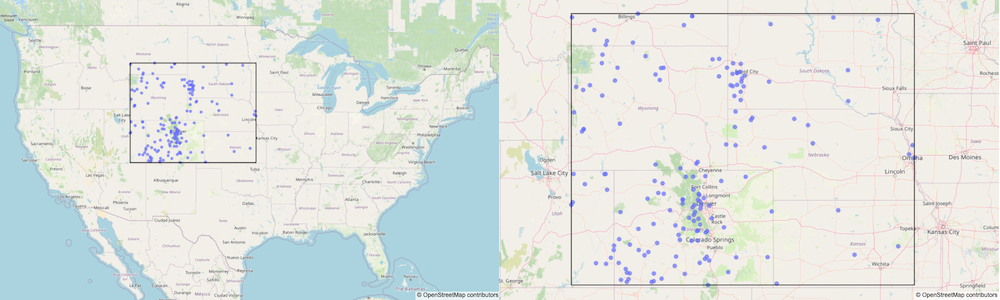
\includegraphics[width=12 cm]{Definitions/st_map_combined}
\caption{Rocky Mountain GACC - 161 RAWS with valid data from 2023 through 2024. (Left) National view, (right) zoomed view\label{fig:st_maps}}
\end{figure}   
\unskip
\subsubsection{Predictors of FMC}
\label{sec:preds}
% Midrule or not?
\begin{table}[tb]
\caption{Predictors Summary\label{tab:all_vars}}
\small
\begin{tabularx}{\textwidth}{l l p{4cm} p{1cm} p{1cm} p{1cm}}
\toprule
\textbf{Variable} & \textbf{Units} & \textbf{Description} & \textbf{Mean} & \textbf{Low} & \textbf{High} \\
\midrule
Drying Equilibrium & $\%$ & Derived from RH and temperature. & 15.21 & 1.33 & 36.90 \\
\midrule
Wetting Equilibrium & $\%$ & Derived from RH and temperature. & 13.84 & 0.61 & 34.65 \\
\midrule
Solar Radiation & $kWh/m^2$ & Downward shortwave radiative flux. & 220.99 & 0.00 & 1130.00 \\
\midrule
Wind Speed & $m/s$ & Wind speed at 10m. & 4.70 & 0.13 & 32.50 \\
\midrule
Elevation & meters & Height above sea level. & 1859.86 & 304.80 & 3521.96 \\
\midrule
Longitude & degree & X-Coordinate & -104.78 & -110.93 & -95.85 \\
\midrule
Latitude & degree & Y-Coordinate & 40.90 & 37.09 & 45.99 \\
\midrule
Rain & mm/h & Calculated from rain accumulated over the hour. & 0.04 & 0.00 & 68.29 \\
\midrule
Hour of Day & hours & From 0 to 23, UTC time. & 11.50 & 0.00 & 23.00 \\
\midrule
Day of Year & days & From 0 to 365 or 366 (leap year in 2024) & 197.00 & 1.00 & 366.00 \\
\bottomrule
\end{tabularx}
\end{table}

For the ML models used in this project, we select a set of predictors of FMC that include atmospheric weather data as well as geographic features of the physical RAWS locations. The set of predictors was chosen based on the typical inputs to various physics-based models of FMC. The final set of predictors is shown in Table \ref{tab:all_vars}. Individual RAWS report spatial coordinates including longitude, latitude, and elevation above sea level in meters. These three spatial characteristics are used as predictors in the RNN and XGBoost models. 

The weather variables were collected from the HRRR, a product developed by NOAA~\citep{Dowell-2022-THR}, using the python software package Herbie~\citep{Blaylock-2024-HRM}. The HRRR model provides real-time, hourly forecasts of many weather variables on a 3km resolution grid across CONUS. All weather variables used in this project were extracted from HRRR version 4, which was introduced in December 2020~\citep{Dowell-2022-THR}. Every 6 hours, the model provides forecasts 48 hours into the future. The HRRR model can therefore be used within a real-time forecasting tool for FMC. \citet{Schreck-2023-MLV} used the HRRR in their FMC modeling project, and the HRRR is used initialize simulations in the WRF-SFIRE project. We retrieve predictors at a given time from the $3^{\text{rd}}$ HRRR forecast hour for the corresponding time 3 hours in the past. The $3^{\text{rd}}$ forecast hour is used for two reasons. First, certain modeled variables, such as wind, tend to be very smooth spatially at the zero hour of the model, and these variables begin to develop a more realistic structure by the third hour. Second, rainfall is one of the key predictors of FMC and the zero hour of HRRR forecasts always has zero precipitation accumulated. We use rainfall in units of accumulated millimeters per hour, since the ODE+KF uses rainfall data with these units. Also, there are ground-based rainfall capture sensors that update hourly on some RAWS, which can be used as a quality control check for HRRR model output for rain. Calibration efforts within the WRF-SFIRE project settled on using the $3^{\text{rd}}$ HRRR forecast hour, when available, instead of the zero hour model. The HRRR weather variables at a given time are interpolated linearly to the location of the RAWS and joined to the FMC data by location and time. 

The air temperature and RH at 2m height from HRRR are used to calculate wetting and drying equilibrium moisture content ($E_d$ and $E_w$), in units of percent FMC (or unitless depending on convention)~\citep[Eqs.\ 4 and 5,][]{VanWagner-1985-EFP}. Downward shortwave solar radiative flux (DSWRF) at the surface is collected from HRRR, in units $W m^{-2}$. DSWRF is a type of solar radiation used by several physics-based models of FMC, including \citet{Nelson-2000-PDC} and \citet{vanderKamp-2017-MFS}. Some RAWS have pyranometers which measure DSWRF and can be used as a quality control check. The rain in terms of $mm\,hr^{-1}$ is calculated from HRRR by subtracting the accumulated precipitation at the $3^{\text{rd}}$ HRRR forecast hour with the accumulated precipitation from the $2^{\text{nd}}$ forecast hour. Some RAWS have rain capture buckets that produce observations hourly accumulated rainfall, which be used as a quality control check for the hourly rain forecasts. Finally, wind speed at 10 meters is collected from HRRR, in units of $m\,s^{-1}$. Some RAWS also have wind sensors positioned at a sampling height of 20 feet, which can be used for validation of the HRRR wind speed data.

Lastly, we utilize two predictors derived from the time of the observations. The hour of the day (0-23 UTC) and the Julian day of the year (0-365 or 366 for leap years) are used as predictors in the ML models. The hour of the day is used to help the ML models capture diurnal cycles in FMC. FMC is the highest at night just after when the humidity is highest and temperature is lowest. The relative position of the sun is a physical driver of the process, so the hour of the day is used as a proxy for the sun position. The day of the year is used to help the ML models capture seasonal affects.

All predictor data was scaled before being input into the ML models. Scaling inputs can lead to improved performance for neural networks. Standard scaling was used, which consists of subtracting the sample mean and dividing by the sample standard deviation for each predictor variable. The mean and standard deviation used for scaling was calculated only on training sets and then applied to testing data. See Section \ref{sec:cv} for more information on the spatiotemporal cross-validation method used in this paper. The response variable of FMC was left unscaled.
\subsubsection{Data Collection Summary}
We collected all available FMC data for 2023 through 2024 within the Rocky Mountain Geographic Area Coordination Center (GACC). The spatial bounding box for this region is from Latitude 37 N to Latitude 46 N, and from Longitude -111 W to Longitude -95 W. This region includes parts of Colorado, Wyoming, Nebraska, Kansas, Montana, and South Dakota. There were 161 total RAWS with valid FMC data in this period and spatial domain, and 151 total RAWS with valid data in the forecasting period of 2024. Figure~\ref{fig:st_maps} shows the location of the RAWS within the Rocky Mountain GACC with valid FMC data from 2023-2024. This region is particularly prone to wildfire danger and numerous federal, state, and local agencies are involved with wildfire management. The atmospheric weather predictors were chosen based on physical considerations and based on inputs to other models of FMC in the scientific literature. A complete list of all data variables used in this study is listed in Table \ref{tab:all_vars}.


\subsection{Recurrent Neural Networks}
\label{sec:rnns}
Recurrent neural networks (RNNs) are a class of neural network architectures that are specific to processing sequence data, where predictors and outcomes are ordered in time. An RNN cell is a basic processing unit where the output at a given time is a function of the input and the output of the cell at previous times~\citep[p.\ 498-501,][]{Geron-2019-HOM}. The simple RNN cell takes as input the set of predictors at time $t$, denoted $X_t$, as well as the output of the recurrent connection at the previous time step, which we refer to in this paper as the ``recurrent state''. The right-hand side of Figure~\ref{fig:rnn} shows the computational flow in a single recurrent unit. The input $X_t$ and the recurrent state $h_{t-1}$ are combined in a linear combination with fixed weights $W_x$, $W_h$ and $b$. This linear combination is modified by an activation function, denoted $\sigma$, to produce the cell output, which in the simple RNN cell is stored as the new hidden state. 
\begin{linenomath}
\begin{equation}
\label{eq:rnn_eq}
    h_t = \sigma(W_x X_t + W_h h_{t-1} + b)
\end{equation}
\end{linenomath}
The weight vector $W_x$ is the same length as $X_t$, which represents input. The weight $W_h$ and the bias $b$ are scalar values. For the simple RNN cell, the output is the same as the new recurrent state. 

Figure~\ref{fig:rnn_flow} shows the recurrent unit ``unrolled'' in time, where the same computational unit is applied recursively. Over time, the recurrent state is modified, but the same set of weights and biases are used at each time step. 

\begin{figure}[tbh]
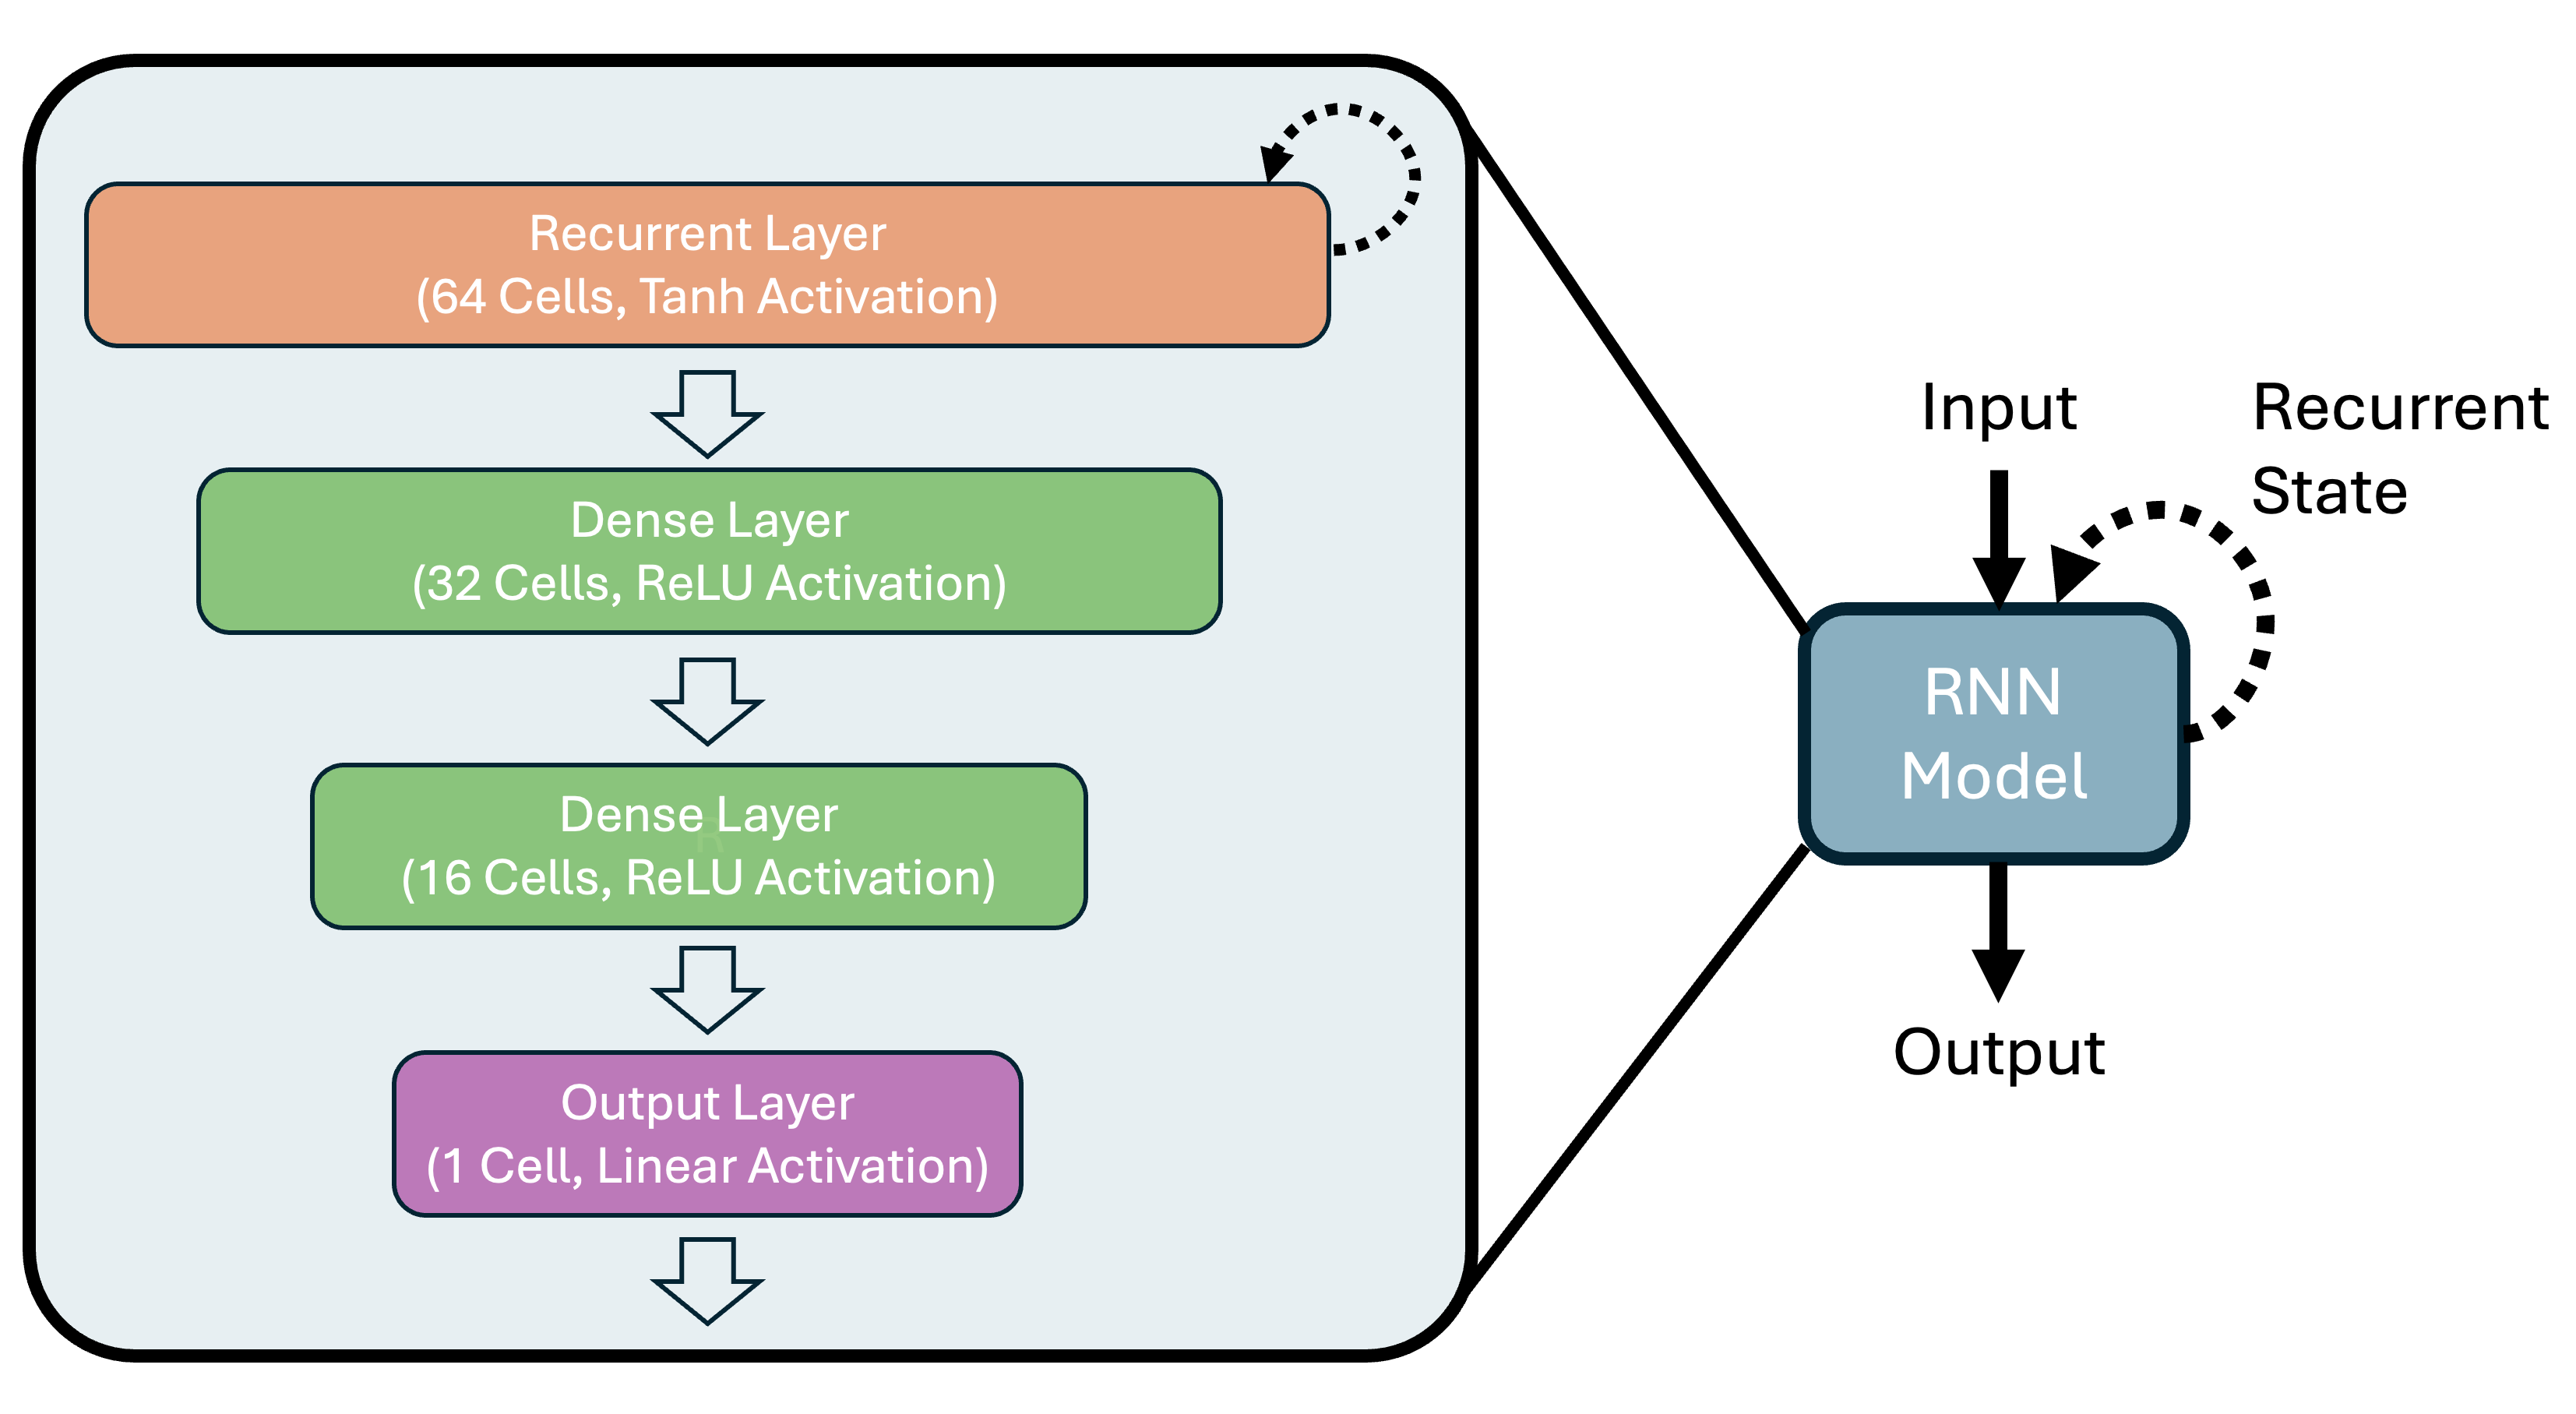
\includegraphics[width=12 cm]{Definitions/rnn1}
\caption{A single recurrent unit takes as input weather data and a recurrent state (left). An LSTM layer and subsequent dense layers forms the recurrent unit (right).}
\label{fig:rnn}
\end{figure}   

\begin{figure}[tbh]
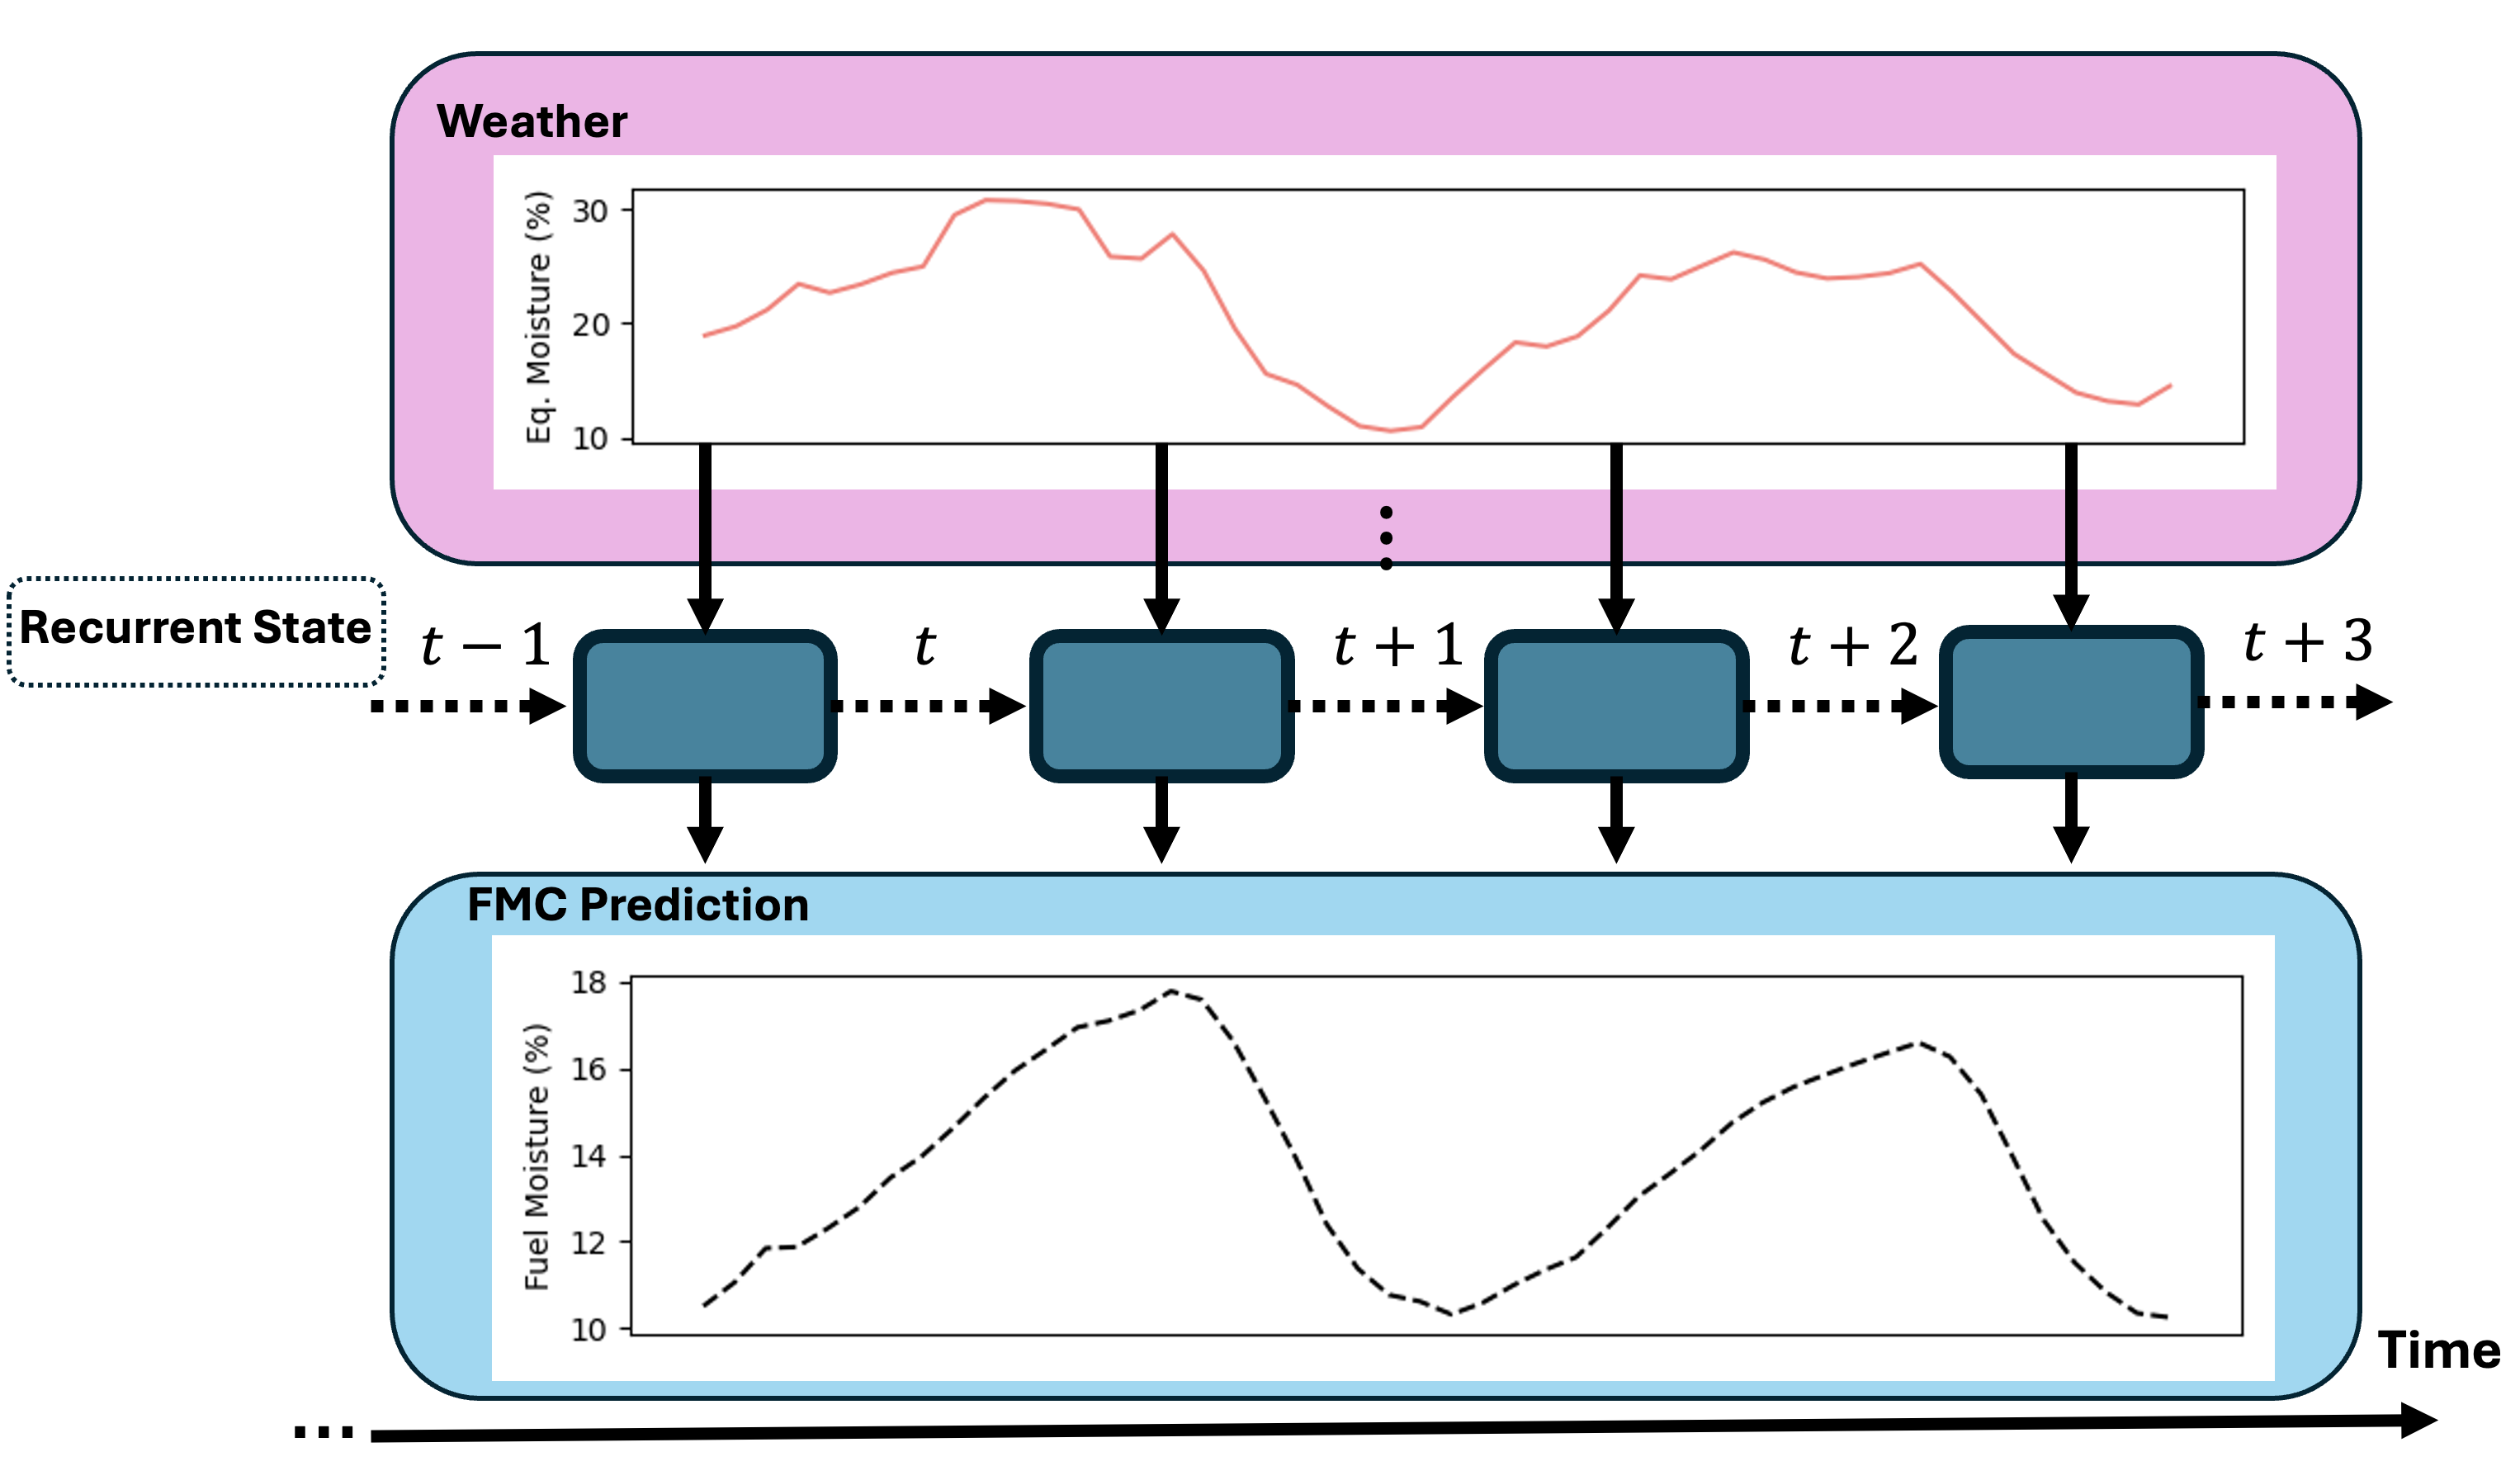
\includegraphics[width=12 cm]{Definitions/rnn_flow}
\caption{The recurrent unit unrolled in time. The recurrent unit with fixed parameters is applied at each time step, and a recurrent state is maintained over time. The output is a mapping of weather inputs to the FMC at the same time.}
\label{fig:rnn_flow}
\end{figure}   

Multiple recurrent cells are typically stacked into a ``recurrent layer''. One or more recurrent layers are used in conjunction with other neural network layers, such as the standard fully-connected ``dense'' layer. We will refer to an ``RNN'' as any neural network architecture with one or more recurrent layers.

A popular type of recurrent model architecture is Long Short-Term Memory (LSTM) (Figure~\ref{fig:lstm_cell}), which was originally developed to address certain issues with the simple RNN cell~\citep{Hochreiter-1997-LST}. Like the simple RNN cell, the LSTM cell maintains a hidden state, which is the output of the cell at the previous time step. In addition to the hidden state, an LSTM maintains a ``cell state'', denoted $c_t$, which incorporates information about the output of the cell over more time steps in the past than just the previous time step. At time $t$, the hidden state $h_{t-1}$ and the predictors $X_t$ are used to modify the cell state through a series of computational gates. The resulting cell state $c_t$ can be viewed as a compromise between the old information as represented by the cell state $c_{t-1}$ and the new information as represented by $h_{t-1}$ and $X_t$. The final output of the cell at time $t$ is a combination of $h_{t-1}$, $X_t$, and $c_t$. This is stored as the new hidden state at time $t$, or $h_t$. LSTM cells are typically stacked into an LSTM layer that is combined with other neural network layers to form a~more complicated model architecture. We will refer to a ``LSTM'' as any neural network that contains one or more LSTM layers. The computational graph in Figure~\ref{fig:rnn_flow} still applies to the LSTM cell, with the modification that the state passed recursively in time to the unit consists of both the hidden state and the cell state, and the output of the unit is the hidden state. For the LSTM cell, the combination of the hidden state and the cell state is the recurrent state.

\begin{figure}[tbh]
\hspace*{0.75cm}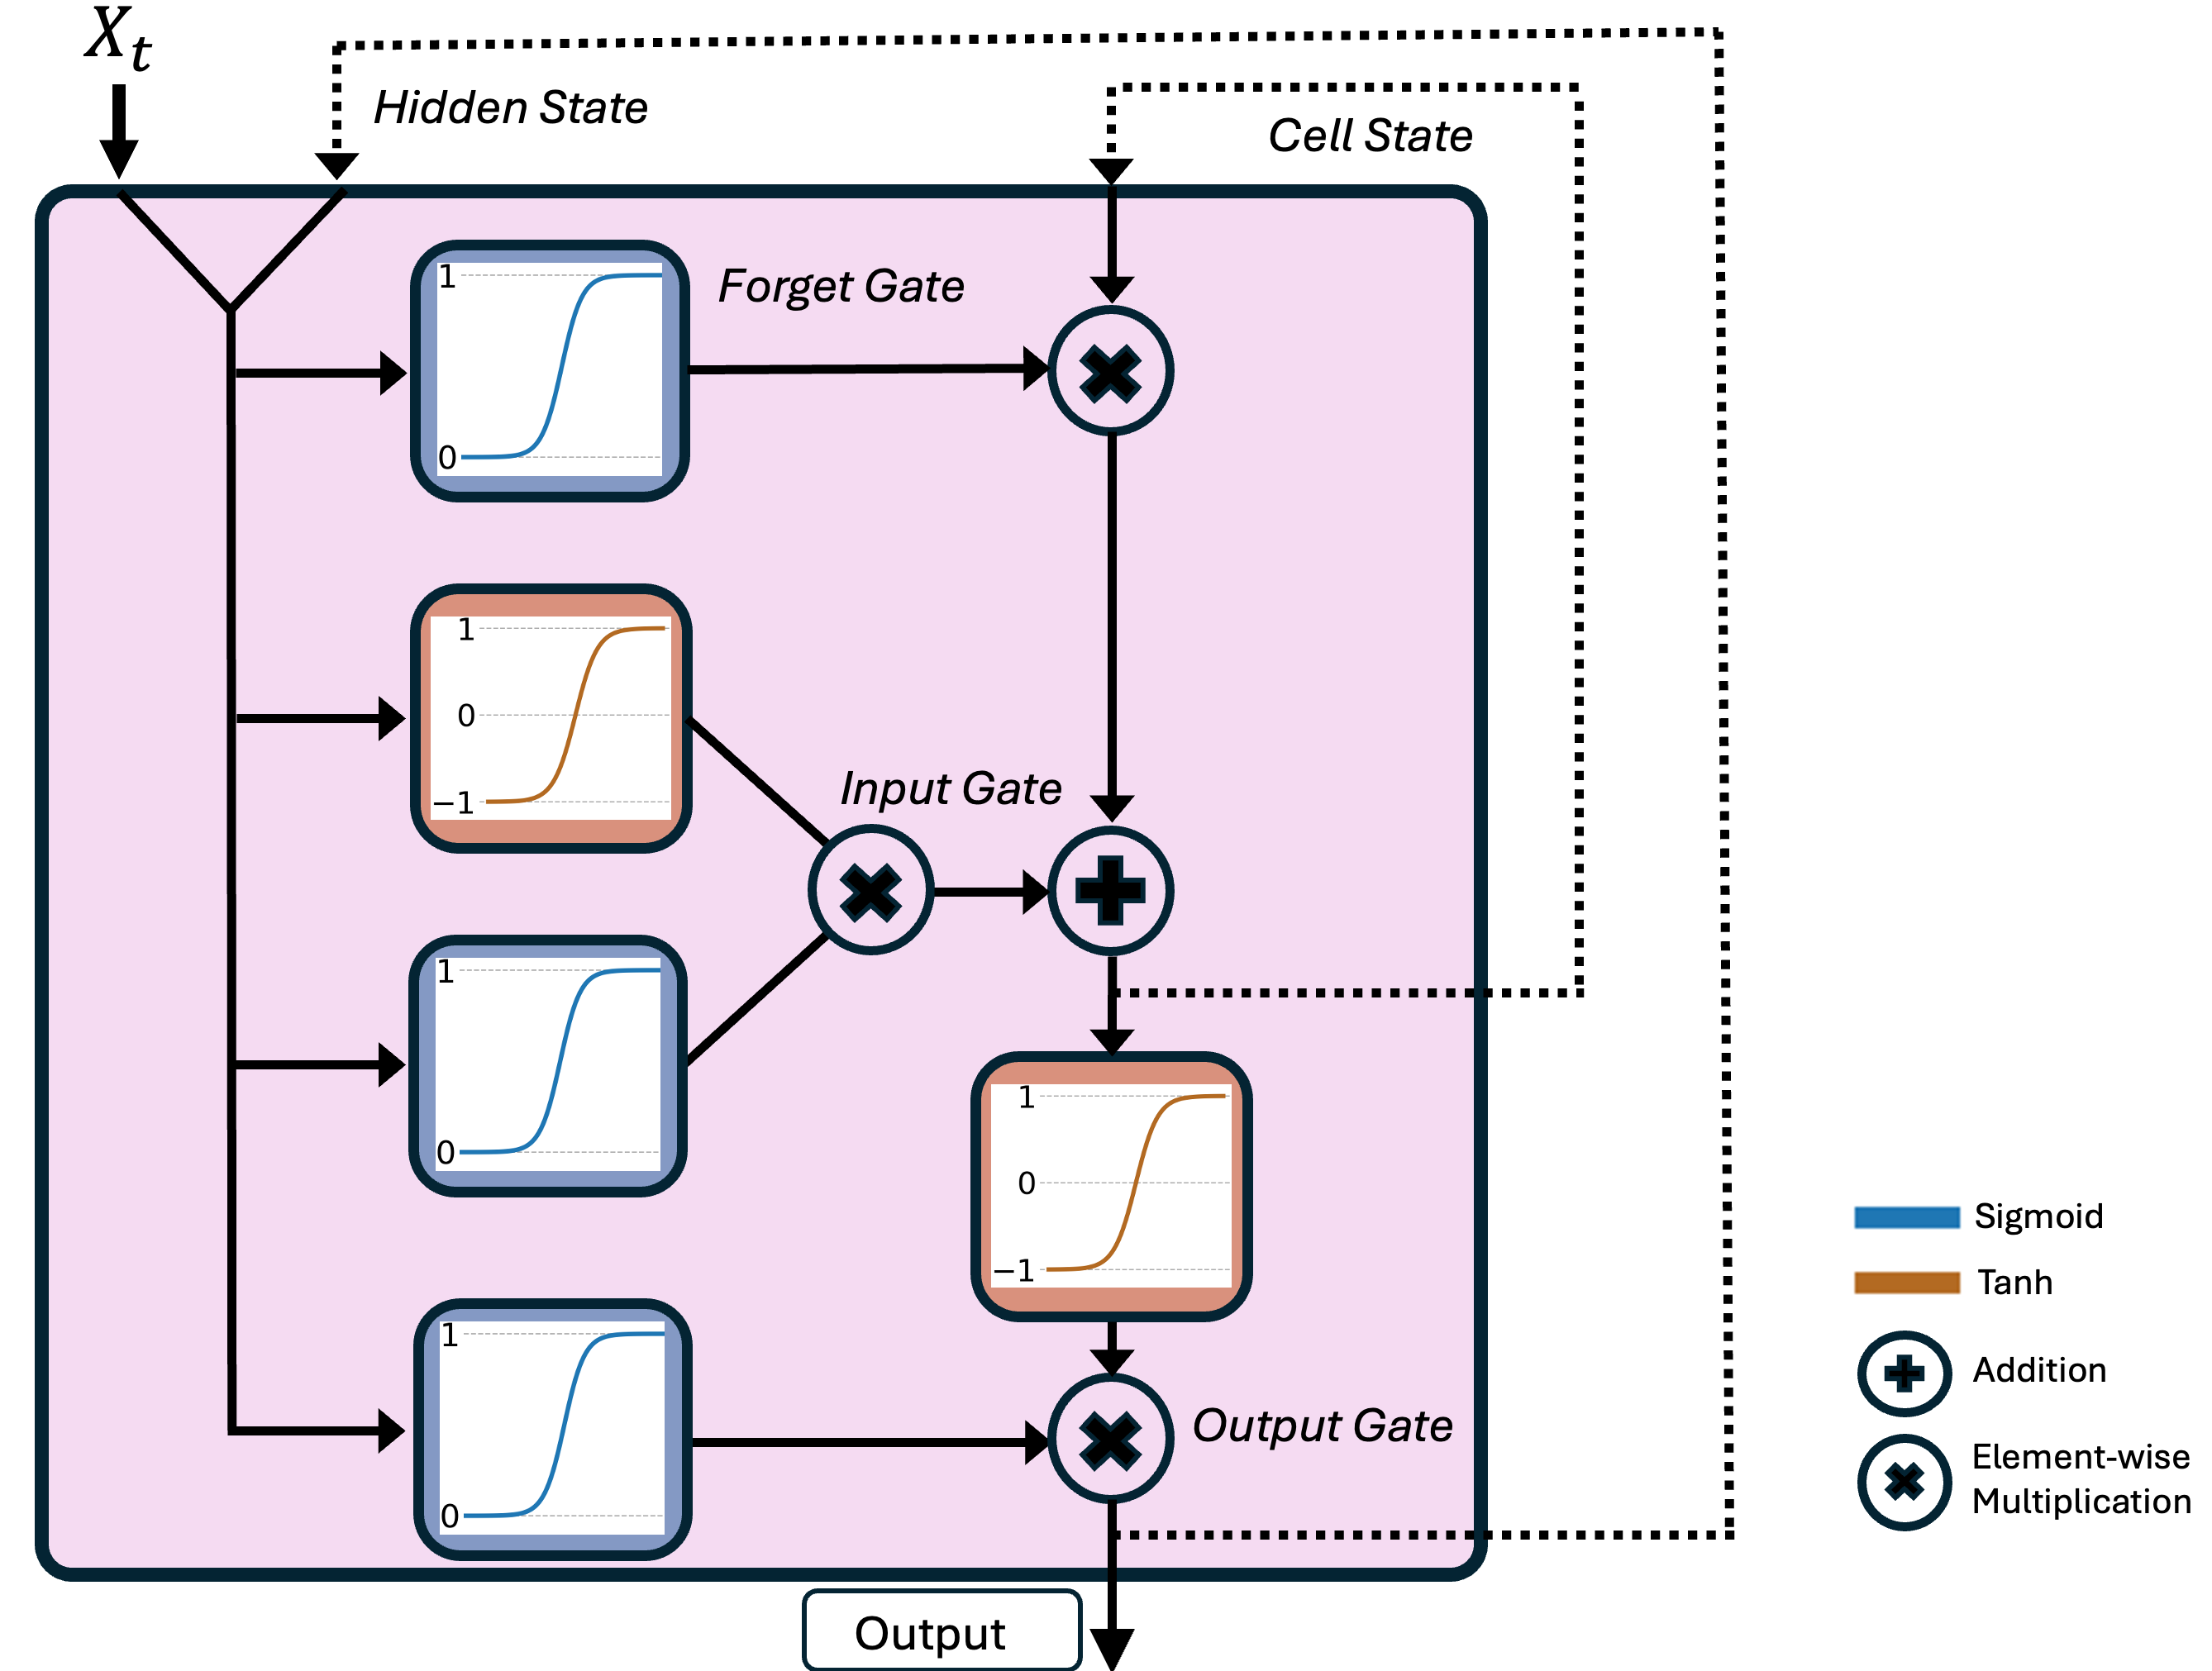
\includegraphics[width=12 cm]{Definitions/lstm_cell}
\caption{A single LSTM cell. (Adapted  from \citet[p. 569,][]{Geron-2019-HOM}.)}
\label{fig:lstm_cell}
\end{figure}   

In this paper, an RNN is trained to map time series of weather variables to time series of FMC, processing one time step at a time. The weather inputs at time $t$ not only result in a predicted FMC at the same time $t$, but also modify the recurrent state, and thus affect the predicted FMC at future times $t+1$, $t+2$,\dots\ Since numerical weather forecasts are used as inputs, it is assumed that the weather is known in the future.

Neural networks contain many parameters that are fitted using a training set by an attempt to minimize a loss function of the model when compared to the observed data. With RNNs, the loss can be computed over time, so the model can learn to minimize the prediction error over a forecast window. During training, a fixed number of time steps, called the sequence length, is used to calculate the loss. 

\begin{figure}[tbh]
\hspace*{2cm}
\includegraphics[width=8 cm]{Definitions/loss}
\caption{Example of predicted versus observed timeseries of FMC.\label{fig:loss}}
\end{figure}   

We use the mean squared error (MSE) as a loss function, which is standard in machine learning for a continuous response. Suppose that an input sequence is of length $T$. The predicted FMC at time $t$ is denoted $\hat y_t$, and the observed FMC at time $t$ is $y_t$. The loss for a single sequence is

\begin{linenomath}
\begin{equation} 
\label{eq:loss} 
    \text{MSE} = \frac{1}{T}\sum_{t=1}^T (y_t - \hat y_t)^2,
\end{equation}
\end{linenomath}
Loss is calculated by comparing the predicted time series of FMC to the observed values (Figure~\ref{fig:loss}).

\subsection{RNN Training, Prediction, and Tuning}
\label{sec:training}

We trained a recurrent neural network (RNN) with gradient descent using the Adam optimizer. Inputs combine time-varying meteorological variables with static spatial features (longitude, latitude, elevation). The target variable is the 10-h dead fuel moisture content (FMC) measured at Remote Automated Weather Station (RAWS) sites.

Training data are arranged as a tensor of shape \texttt{(batch size, sequence length, features)}. Here, features is the number of unique inputs. Following~\citet[Sect.~9.7]{Zhang-2023-DDL}, we use truncated backpropagation through time (BPTT). A single sample consists of a tensor of shape \texttt{(sequence length, features)}. At the start of processing a sample, the recurrent state is reset. At each time step of the sample, a one-dimensional tensor of features is input to the model, the recurrent state is updated, and a single output is generated. This process is repeated for the entire sample. The output of the network from an entire sample is a timeseries of FMC predictions of the same sequence length as the input sample, which requires setting the function argument \texttt{return\_sequences} to true~\citep{Keras-2025-LSTM}. The model loss for the sample is the MSE, as seen in Equation~\ref{eq:loss}, averaged over the entire sequence length. The gradient of the loss with respect to all model parameters is then calculated via BPTT. Gradients are calculated for each sample sequence in a batch and then averaged across samples~\citep{Keras-2025-Loss}. Model parameters are updated after each batch. A single epoch of training is completed when all batches of samples have been processed. Early stopping halts training when validation performance no longer improves. 

The static predictors are repeated at each time step. Batches include samples from multiple locations to promote generalization and learn the dependence on location. The model parameters are updated after each batch.

During training, the effective temporal depth of optimization is limited by the sequence length and batch size. Consequently, truncated BPTT is applied only within this finite window, ensuring computational stability~\citep[Sect. 9.7.1.2]{Zhang-2023-DDL}. In contrast, during prediction, the model operates with an unconstrained sequence length and a batch size equal to the unique number of locations for prediction, receiving new weather inputs sequentially and updating its recurrent state indefinitely. The prediction process is therefore equivalent to unrolling the RNN for an arbitrary number of time steps without truncation, allowing the model to integrate meteorological history over potentially long periods. The same network parameters, trained within the finite truncated BPTT horizon, are reused for recursive forecasting by copying the learned weights from the training configuration to the stateful inference model~\citep[p.~512]{Geron-2019-HOM}.

Neural networks have many fixed hyperparameters, such as the number of cells to use within a layer, the overall number of layers, the batch size, the learning rate, etc. It is important to keep the data used to tune hyperparameters separate from data used to estimate forecast accuracy. The metrics calculated on forecasts should represent the accuracy of the model when predicting entirely new data. The hyperparameter tuning used in this project will be described in Section \ref{sec:cv}.

\subsection{Recurrent Neural Network for Forecasting FMC}
\label{sec:model}
In this paper, we use the following RNN model architecture. The input is a collection of features consisting of weather variables and geographic locations of RAWS. These inputs are fed into a single LSTM layer consisting of 64 cells with hyperbolic tangent activation function. The LSTM layer outputs a sequence of the same length as the input data, and the entire sequence is passed through the network until the output layer. The output of the LSTM layer is fed into two dense, fully connected layers with ReLU activation and 32 and 16 cells, respectively. The LSTM layer and the dense layers process each time step in the sequence independently. Finally, the output of the model is a single neuron with linear activation. Linear activation is chosen for the final output layer, since we are mapping the inputs to a continuous real number. A single neuron is used as an output layer since model predictions are generated by deploying the model point-wise at each location, and thus the FMC at a given time is considered to be a single scalar value. The final model output is a two-dimensional vector, where the first dimension is the number of unique locations and the second is the number of time steps (48 hours in our case). Other model architectures can be used to generate outputs that correspond to a spatial grid, but we chose this architecture since it is the easiest to implement and is the most flexible when predicting across various spatial domains. The left side of Figure~\ref{fig:rnn} shows a diagram of the architecture of the RNN model used in this study.  

The HRRR model is used to provide weather input to the RNN. HRRR provides hourly forecasts up to a maximum of 48 hours. The sequence length used to structure the data input \texttt{(batch size, sequence length, features)}, described in Section \ref{sec:rnns}, is set to 48. Each input to the RNN consists of a 48-hour sequence of observations, and every output of the model is a 48-hour sequence of FMC predictions at the same times as the input. The batch size is a tuned hyperparameters, and the number of features was determined through theoretical considerations described in Section \ref{sec:preds}. 

In this study, we evaluate the forecast accuracy over all of year 2024 broken into 48 hour periods to align with the sequence length of training inputs. The initial hidden state and cell state of the LSTM layers are zero by default. Starting at 00:00 UTC on January 1, 2024, we input 48 hours of HRRR weather data and geographic input at a given set of test locations to generate the first set of forecasts. Then, for the next 48 hours, the initial hidden state and the cell state of the LSTM are reset. This process is repeated until all 2024 forecasts are generated. The initial recurrent state of the LSTM is reset for each 48-hour forecast period and no information is retained across distinct forecasting periods. Resetting the recurrent state in this way is done for the purposes of estimating the forecast accuracy of the model 48 hours into the future. Resetting the recurrent state is not required for this model architecture, and an operational version of the model could retain the recurrent state for arbitrarily long.

The hyperparameters for the RNN were selected with a restricted grid search, which evaluates a subset of all possible hyperparameter combinations. The combination of hyperparameters that leads to the most accurate predictions on the validation set is chosen. Here, some hyperparameters were set to their default values from the TensorFlow software project, which are generally accepted in the literature as reasonable defaults. Table \ref{tab:rnn_params} shows the hyperparameters used in the model that are not part of the core model architecture shown in the left-hand side of Figure~\ref{fig:rnn}. The hyperparameter tuning method is discussed in Section~\ref{sec:cv}, and Appendix~\ref{sec:appendix_hyper} has additional technical details.

\begin{table}[tbh]
\small
\caption{RNN Hyperparameters\label{tab:rnn_params}}
\begin{tabularx}{\textwidth}{CCC}
\toprule
\textbf{Hyperparameter} & \textbf{Value} & \textbf{Description} \\
\midrule
Learning Rate & 0.001 & Controls how fast weights update during training \\
\midrule
Timesteps & 48 & 
% Number of timesteps for each input 
Sequence size\\
\midrule
Batch Size & 64 & Number of sequences to process before updating weights \\
\midrule
Dropout & 0.15 & Rate that weights are randomly set at during training \\
\midrule
Early Stopping Patience & 5 & Number of epochs with no improvement to validation error before stopping training \\
\midrule
Scaling & Standard & Scaling inputs to mean zero and std. 1 \\
\bottomrule
\end{tabularx}
\end{table}

\subsection{Baseline Methods}
\label{subsec:baseline}

\subsubsection{ODE model with Kalman Filter in WRF-SFIRE}
\label{sec:ODE_KF}
The ODE+KF uses a first-order timelag differential equation with data assimilation~\citep{Mandel-2014-RAA, Vejmelka-2016-DAD}. This model uses drying and wetting equilibrium moisture content and hourly accumulated rainfall as input. Data assimilation of FMC observations from RAWS is done using the augmented Kalman filter~\citep{Vejmelka-2016-DAD}. During wildfire simulations, WRF-SFIRE receives the initial fuel state from the ODE+KF after data assimilation, and then the ODE model inside WRF-SFIRE runs in forecast mode without data assimilation to update the FMC throughout the duration of the simulation. Model calibration was performed using wildfire simulations from WRF-SFIRE, comparison to the fine fuel moisture model from the Canadian fire danger rating system~\citep{VanWagner-1985-EFP}, and comparison to RAWS in Colorado and the Pacific Northwest. Equation \ref{eq: ode} describes the mathematical form for $m(t)$, the FMC at time $t$:
\begin{equation}
\label{eq: ode}
    \frac{d}{dt}m(t) = \begin{cases}
        \frac{S-m(t)}{T_r}\left(1-\exp\left(\frac{r_0 - r(t)}{r_s}\right)\right) & \text{if}\;\; r(t) > r_0 \text{ (soaking in rain)}\\
        \frac{E_d(t)-m(t)}{T_k} & \text{if}\;\; r(t)\leq r_0 \text{ and }m(t)>E_d(t)\\
        \frac{E_w(t)-m(t)}{T_k} & \text{if}\;\; r(t)\leq r_0 \text{ and } m(t)<E_w(t)\\
        0 & \text{if}\;\; r(t)\leq r_0 \text{ and } E_w(t)\leq m(t)\leq E_d(t)
    \end{cases}
\end{equation}
If the amount of rainfall accumulated per hour $r(t)$ is greater than the threshold value $r_0$, it is assumed that the stick absorbs water directly, and it approaches a saturation moisture level $S$ with a characteristic delay time depending on rain intensity, asymptotically $T_r$ for a very intense rain. The saturation rainfall intensity $r_s$ is when rain wetting is $1-e^{-1}\approx 63\%$ of the maximal rate. The calibration of the model resulted in a threshold rainfall intensity of $r_0=0.05 \, mm\,h^{-1}$, a saturation level $S=250\%$, a delay time $T_r = 14\,h$, and a rain saturation intensity of $r_s=8 \,mm\;h^{-1}$~\citep{Mandel-2014-RAA}. These values will be referred to as hyperparameters for consistency with other models. If the rainfall $r(t)$ is less than the threshold value $r_0$, the stick changes moisture by equilibrating to the equilibrium moisture content of the surrounding environment. There are three distinct dynamics for the FMC in no-rain conditions. If the FMC $m(t)$ is greater than the current drying equilibrium moisture content $E_d(t)$, then drying dynamics occur and the FMC approaches $E_d(t)$ with a characteristic time-lag of $T_k$ determined by the fuel class ($T_k$ = 10 for 10-h fuels). If $m(t)$ is less than the current wetting equilibrium moisture content $E_w(t)$, then wetting dynamics occur and the FMC approaches $E_w(t)$ with the same characteristic time-lag of $T_k$. If $m(t)$ is between $E_d(t)$ and $E_w(t)$, there is no change in moisture content. We use the ODE+KF with the calibrated parameters described above to forecast the FMC at the locations not included for training the ML models and at times in the future of all ML training data. The ODE equations described above can be solved analytically, and a discretized version of the analytic solution is used to model FMC.

In the model by \citet{Vejmelka-2016-DAD}, the state of the system was extended to include an equilibrium bias correction to allow the model to learn differences between the equilibrium moisture content values as determined by laboratory experiments versus what is suggested by the data. In this paper, a spinup period of 24 hours is used for the equilibrium bias correction to stabilize. The spinup period is the number of time steps where data assimilation via the Kalman Filter occurs. After 24 hours of spinup, the model is run in forecast mode for 48 hours. In forecast mode, the model receives weather inputs, but no input from observed FMC. 

In \citet{Vejmelka-2016-DAD}, a spatial regression procedure is used to interpolate FMC observations from RAWS to a computational grid, and the interpolated FMC values are used for data assimilation into the ODE+KF model running on each grid node. 

Here, since we are interested in a comparison at the locations of the RAWS in the test set, we run ODE+KF at those RAWS locations, and assimilate the RAWS FMC data directly.
Table \ref{tab:ode_params} shows a summary of the hyperparameters used within the ODE+KF.

\begin{table}[tbh]
\caption{ODE+KF Hyperparameters\label{tab:ode_params}}
\small
\begin{tabularx}{\textwidth}{CCC}
\toprule
\textbf{Hyperparameter} & \textbf{Value} & \textbf{Description} \\
\midrule
Spinup & 24 & Number of hours to run model with data assimilation \\
\midrule
Process Variance & 1e-3 & Uncertainty in model dynamics \\
\midrule
Data Variance & 1e-3 & Uncertainty in measurement of input data \\
\midrule
$r_0$ & 0.05 & Threshold rainfall intensity ($mm h^{-1}$) \\
\midrule
$r_s$ & 8.00 & Saturation rainfall intensity ($mm h^{-1}$) \\
\midrule
$T_r$ & 14.00 & Characteristic decay time for wetting dynamics ($h$) \\
\midrule
$S$ & 250 & Saturation FMC level \\
\midrule
$T$ & 10.00 & Characteristic decay time for fuel class \\
\bottomrule
\end{tabularx}

\end{table}

\subsubsection{The XGBoost Static Model}
The ML model used as a baseline is an implementation of the Extreme Gradient Boosting (XGBoost) technique~\citep{Chen-2016-XAS}, which has been used by FMC researchers in recent years~\citep{Schreck-2023-MLV}. The XGBoost uses ensembles of regression trees that are iteratively fit and re-weighted. XGBoost produces a nonlinear model which is a weighted average of regression trees, resulting in a piecewise-constant mapping of the predictors to the output. Our implementation of XGBoost is ``static'', or nonrecurrent, meaning that the model is learning a map between the predictors and the observed FMC at a~moment of time and incorporating no information about the FMC at previous times. Thus, the instantaneous relationship between the predictors and the response is learned, and observations of FMC are implicitly considered independent in time. Time-based predictors are utilized in our implementation of the model, such as the hour of the day and the day of the year, but the model is still nonrecurrent since the output at a given time step is not a function of the output at the previous time step. Hyperparameters for the XGBoost model were based on previous work by \citet{Hirschi-2025-CLF}, where various static ML models were tested over 2023 in the Rocky Mountain region. Table \ref{tab:xgb_params} shows a summary of the hyperparameters used within the XGBoost model.

\begin{table}[tbh]
\caption{XGBoost Hyperparameters}
\label{tab:xgb_params}
\small
\begin{tabularx}{\textwidth}{CCC}
\toprule
\textbf{Hyperparameter} & \textbf{Value} & \textbf{Description} \\
\midrule
N Estimators & 100 & Number of trees in ensemble \\
\midrule
Max Tree Depth & 3 & Maximum tree depth. \\
\midrule
Learning Rate & 0.10 & Controls how fast weights update during training \\
\midrule
Min Child Weight & 1 & Minimum sum of Hessian of samples in a partition \\
\midrule
Gamma & 0.10 & Minimum loss reduction required for a tree partition \\
\midrule
Subsample & 0.80 & Percent of training data randomly selected in each boosting iteration \\
\midrule
Colsample by Tree & 0.90 & Percent of predictors randomly selected in each boosting iteration \\
\bottomrule
\end{tabularx}
\end{table}

\subsubsection{Climatology Method}
Lastly, we utilize a climatology method. In weather forecasting, climatology refers to simple statistical methods in which historical weather patterns are used to predict new values of a particular variable. We utilize a climatology method for FMC that is based on a method used by~\citet{Schreck-2023-MLV}. Given a particular time and location, the hour of the day (0-23 UTC) and the Julian day of the year (0-365 or 366) are extracted. The FMC forecast for that hour and location is the historical average of the FMC at that exact location and the same hour of the day, for the days of the year within 15 days of the target time. In this study, we build a climatology by looking back 10 years for each forecast time and location. If there are historical observations from less than 6 unique years at a particular location for a particular time, the FMC forecast was set to missing. These configurations for the climatology method will be referred to as hyperparameters for consistency with the other methods. Table \ref{tab:clim_params} shows a summary of the climatology hyperparameters used in this study.

\begin{table}[tbh]
\small
\caption{Climatology Hyperparameters}
\label{tab:clim_params}
\begin{tabularx}{\textwidth}{CCC}
\toprule
\textbf{Hyperparameter} & \textbf{Value} & \textbf{Description} \\
\midrule
Years & 10 & Number of years to look for historical FMC at a given location \\
\midrule
Days & 15 & Number of days plus or minus the target time to aggregate historical FMC data \\
\midrule
Min. Years & 6 & Minimum unique number of years of observed FMC to generate a prediction \\
\bottomrule
\end{tabularx}

\end{table}

\subsection{Analysis Design}
\label{sec:cv}

We seek to forecast FMC at arbitrary locations in a region where the training FMC data are and at future times. The model maps a time series of weather forecasts to a time series of spatial FMC forecasts based on FMC and weather data that were presented to it during training. In a sense, the model interpolates in space and extrapolates the weather-to-FMC mapping in time. We will compare the models using the root mean squared error (RMSE) at new locations and at times in the future of the times used for training. The RMSE for the FMC models is interpretable in units of percent. In all reported RMSE values in this paper, the square root is applied after any averaging operations; that is, the square root is always the final operation.

Cross-validation methods estimate the accuracy with which a model predicts unseen data~\citep[Sect.~7.10]{Hastie-2010-ESL}. In machine learning, samples are randomly drawn to form independent training, validation, and test sets~\citep[Sect.~7.2]{Hastie-2010-ESL}. The training set is used to fit the model, the validation set to tune hyperparameters and monitor overfitting, and the test set, kept separate, to estimate final predictive accuracy. In time-dependent problems, the test data should come from a period after the training data to reflect the real forecast conditions. This requirement conflicts with the common assumption that training and test samples are independent and identically distributed because temporal ordering introduces dependence. The evaluation of time-series models must therefore balance statistical independence with causal realism. In spatially-dependent problems, the test data needs to be from locations that were not used in training model parameters. If a model is used to predict at locations included in its training data, it has already learned aspects of the data structure at those locations, leading to overly optimistic accuracy estimates~\citep{Schreck-2023-MLV}.

To estimate the forecast error of FMC models at unobserved locations, we apply a spatiotemporal cross-validation procedure. In the hyperparameter tuning step, FMC observations from 2022 are used to train a set of candidate model architectures. A random sample of 90\% RAWS is used to generate the training locations and 10\% to generate the testing locations. Then, the forecast accuracy of those models are compared at the testing locations over all of 2023. During the forecast period, HRRR inputs are used to generate predictions, but no FMC data from the testing time period or testing locations are used to inform predictions. The model architecture with the lowest RMSE when forecasting in 2023 was selected. 

With the model architecture fixed, the model is trained from scratch on observations in 2023 with a random sample of testing locations and training locations. The trained model is used to forecast at locations not used in the training over all of 2024. The final accuracy metrics for the model are calculated by comparing the forecasts from 2024 to FMC observations at the testing locations. The training period always precedes the forecast period in time, and random sampling of locations accounts for spatial uncertainty. A schematic diagram of this cross-validation method is shown in Figure~\ref{fig:cv}, with the training period of 2023 and the forecast period of 2024.

\begin{figure}[tbh]
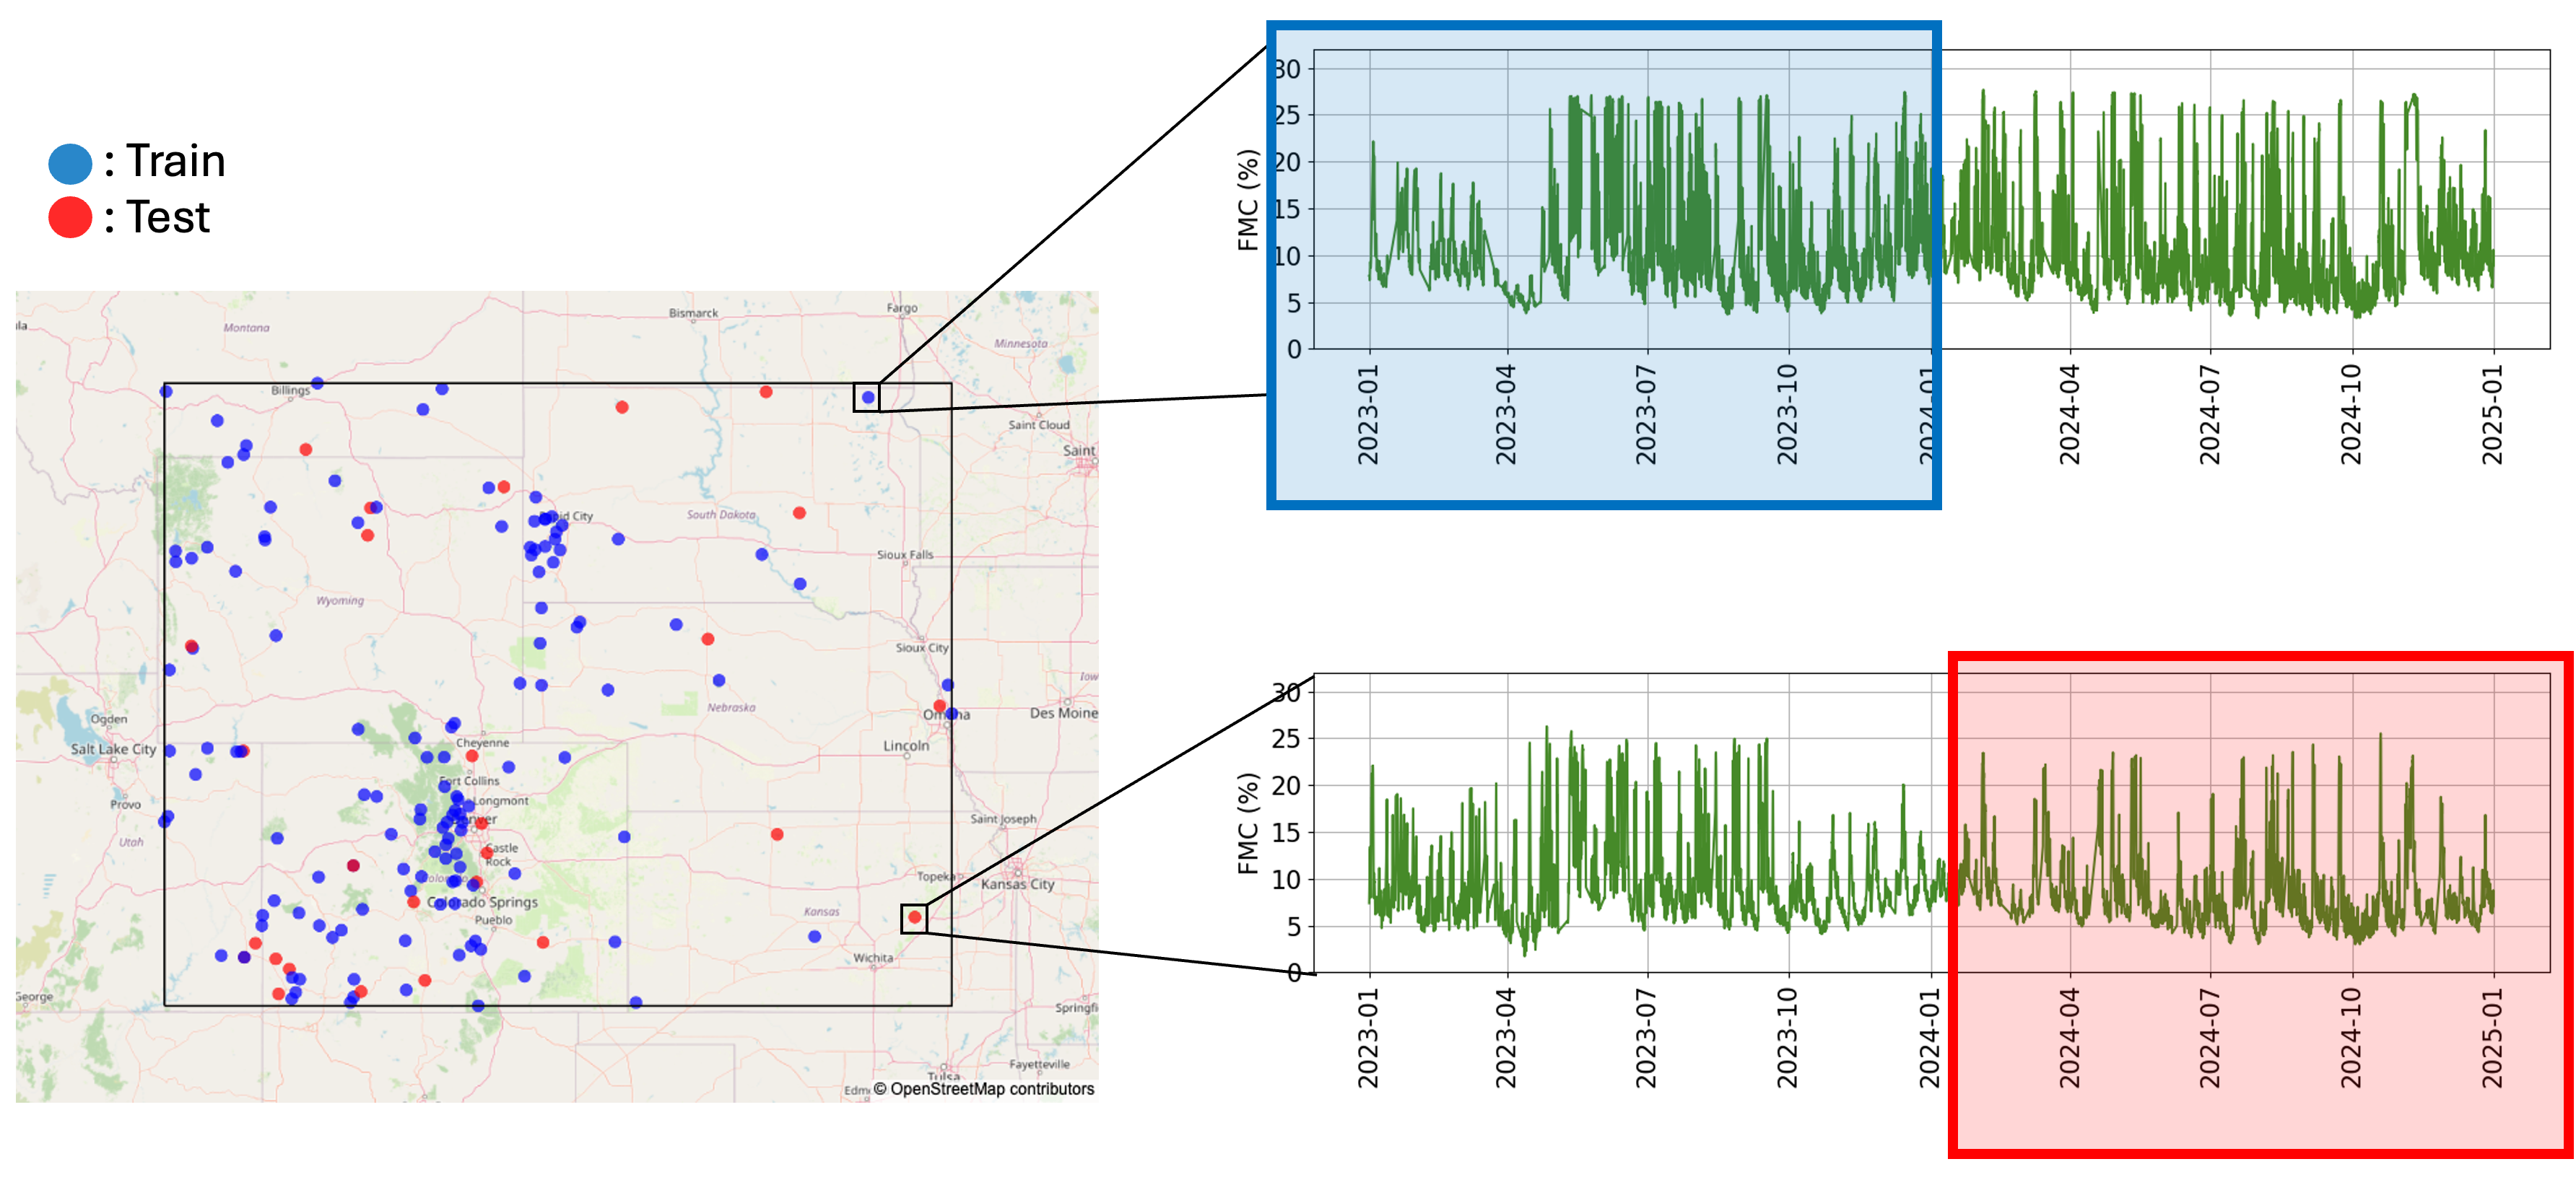
\includegraphics[width=12 cm]{Definitions/cv_diagram}
\caption{Spatiotemporal cross-validation diagram. Spatial locations are randomly sampled for train/test sets (left), and the training period precedes the testing period (right).\label{fig:cv}}
\end{figure}   

The ODE+KF and the climatology methods do not fit directly into the training and testing paradigm used in ML. The ODE+KF is run in forecast mode (i.e. without data assimilation) over all of 2024 at the test locations in 48-hour increments to mimic the initialization with a spinup period. The ODE+KF utilizes 24 hours of data prior to the start of the forecast as a spinup period (i.e. with data assimilation). Each iteration of 24-hour spinup plus 48-hour forecasting were independent. The climatology method produces forecasts by retrieving historical data for each time in 2024 and each testing location. Therefore, the climatology method does not utilize spatial holdout like the ML models, so the accuracy metrics for the climatology method are more optimistic than for the ML methods. 

To account for the variability in the random spatial samples and randomness due to model initialization, the training in 2023 and forecasting in 2024 was repeated 500 times with different random seeds. So, 500 random samples of RAWS were used as training and test splits and 500 different initial weights were used for the ML models. These will be referred to as replications from now on. The replications are used to construct uncertainty bounds on the final accuracy metrics. There were 151 RAWS with valid data in the forecast period of 2024, and each replication had 16 RAWS in the test set, and each RAWS was included in the test set on average 53.0 times in distinct replications.

Within each replication, the forecast residuals are calculated by subtracting the predicted FMC from the observed FMC for each model and at each time. The residual shows whether the forecast was too high or too low and can be positive or negative. We then calculate the squared residual, which is always positive. Within a replication for a given model, squared residuals are calculated across a set of test set locations and a set of forecast times. The per-replication MSE is calculated by averaging the squared residuals over all test locations and test times for a given replication. Then, the overall RMSE is calculated by averaging all the per-replication RMSE values and taking the square root. Uncertainty bounds are calculated from the square root of one standard deviation of the per-replication MSE values. The overall model bias is calculated in the same was using the raw residuals rather than the squared residuals. This metric is used to analyze whether the forecasts are systematically too high or too low. The overall model RMSE and bias are calculated by averaging over all locations and times in the test set. Both the RMSE and bias are interpretable in units of percent FMC. Equation \ref{eq:mse} shows the mathematical form of the RMSE estimate used to quantify forecast error across the entire study region and all times in 2024, using mathematical definitions in Table \ref{tab:defs}. Equation \ref{eq:bias} shows the mathematical form of the bias estimate. Equation \ref{eq:mse_std} shows how the standard deviation of the RMSE is calculated, and the standard deviation of the bias estimate is calculated in an analogous way.

\begin{table}[tbh]
\caption{Mathematical Definitions used for Accuracy Metrics\label{tab:defs}}
\begin{tabularx}{\textwidth}{CCC}
\toprule
\textbf{Term} & \textbf{Description} & \textbf{Data Summary} \\
\midrule
$N$ & Number of unique RAWS & 151 RAWS with FMC data in 2024 in study region \\
\midrule
$T$ & Number of forecast hours & 8,784 hours in 2024 (a leap year)\\
\midrule
$R$ & Number of replications & 500 \\
\midrule
$y_{i,t}$ & Observed FMC at location $i$ and time\textsuperscript{1} $t$ & - \\
\midrule
$y_{r, i, t}$ & Predicted FMC at location $i$, time $t$, and replication\textsuperscript{2} $r$& - \\
\bottomrule
\end{tabularx}
\noindent{\footnotesize{\textsuperscript{1} Observed FMC has no variance across replications.\\ \textsuperscript{2} Predicted FMC has variance across replications due to random selection of stations used in training set and random initializations of the ML model weights.}}
\end{table}
We calculate a per-replication MSE by averaging the squared error over all times and locations,
\begin{linenomath}
\begin{equation}
\label{eq:mser}
    \text{Per-Replication MSE} \equiv \text{MSE}_r = \frac{1}{N\cdot T}\sum_{i=1}^{N} \sum_{t=1}^{T} (y_{i, t} - \hat y_{r, i, t})^2
\end{equation}
\end{linenomath}
The overall RMSE is calculated by averaging the per-replication RMSE over all replications,
\begin{linenomath}
\begin{equation}
\label{eq:mse}
    \text{Overall Mean RMSE} \equiv \overline{\text{MSE}} = \sqrt{\frac{1}{R}\sum_{r=1}^R\text{MSE}_r}
\end{equation}
\end{linenomath}
We estimate the uncertainty in the overall RMSE by calculating the square root of the standard deviation of the MSE across all replications,
\begin{linenomath}
\begin{equation}
\label{eq:mse_std}
    \text{Overall Std. of RMSE} \equiv \sqrt{\frac{1}{R-1} \sum_{r=1}^R\left[\text{MSE}_r - \overline{\text{MSE}}\right]^2}
\end{equation}
\end{linenomath}
We calculate the bias of the models by averaging the error across all times and replications, and the associated standard deviation of the bias is calculated in an analogous way to the standard deviation of the MSE,
\begin{linenomath}
\begin{equation}
\label{eq:bias}
    \text{Overall Bias} \equiv \overline{\text{Bias}} = \frac{1}{R\cdot N\cdot T}\sum_{r=1}^R\sum_{i=1}^{N} \sum_{t=1}^{T} (y_{i, t} - \hat y_{r, i, t})
\end{equation}
\end{linenomath}

We further analyze the forecast error by location and by hour of the day. For the RMSE by hour of the day, model errors are averaged over location, replication number, and days of the year to produce a single RMSE estimate for each hour to analyze how the forecast error changes throughout the diurnal FMC cycle. Further, this analyzes how the accuracy changes as the forecast is run longer into the future. To analyze the spatial variability of the forecast error, the RMSE and bias are calculated by averaging over all times and replications in the test set, producing accuracy metrics for each RAWS. Again, the replications are used to construct uncertainty bounds. Within a single replication we get an estimate of the forecast accuracy for 16 of the total RAWS. After many replications, we end up with estimated RMSE and bias, and uncertainty bounds, for every RAWS with data availability in 2024. The standard deviations of these RMSE estimates across replications are calculated in an analogous way to Equation \ref{eq:mse_std}.  

%%%%%%%%%%%%%%%%%%%%%%%%%%%%%%%%%%%%%%%%%%
\section{Results}
\label{sec:results}

The accuracy of the RNN model and three baseline models was evaluated when predicting values at unobserved locations across all of 2024. The models were evaluated on the same randomly selected test locations across 500 random samples of locations. Table~\ref{tab:overall} shows the RMSE when averaged over all times, locations, and replications. The bounds on the estimated metrics are plus or minus one standard deviation of the given metric across all replications. The RNN achieved the lowest forecast error compared to the baseline methods as indicated by the RMSE. Further, the RMSE of the RNN is well below the uncertainty bounds of the other methods. Thus, there is strong statistical evidence that the RMSE of the RNN is lower than the other methods for the analysis period of 2024 in the Rocky Mountain region. 

\begin{table}[tbh]
\caption{Overall Forecast Error}
\label{tab:overall}
\begin{tabularx}{\textwidth}{CCC}
\toprule
\textbf{Model} & \textbf{Bias (\% FMC)} & \textbf{RMSE (\% FMC)} \\
\midrule
RNN & -0.19 $\pm$ 0.33 & 3.02 $\pm$ 1.12 \\
ODE+KF & -2.41 $\pm$ 0.24 & 4.97 $\pm$ 1.52 \\
XGBoost & -0.4 $\pm$ 0.32 & 4.19 $\pm$ 1.31 \\
Climatology & -0.64 $\pm$ 0.4 & 5.0 $\pm$ 1.46 \\
\bottomrule
\end{tabularx}
\end{table}

A bias of zero would indicate that a model is on average over-predicting FMC just as often as it is under-predicting. Based on the bias metrics and the associated uncertainty, the RNN show signs of being unbiased overall since zero lies within the uncertainty bounds. We examine the RNN errors more closely by stratifying the FMC values into low (0-10\%), medium (10-20\%), and high (+20\%). Table \ref{tab:bias} shows the mean bias and standard deviation for these thresholds, calculated over all 500 replications. Figure~\ref{fig:hists} shows the distribution of observed and predicted FMC.

\begin{table}[tbh]
\caption{RNN Bias by FMC Level.}
\label{tab:bias}
\begin{tabularx}{\textwidth}{CCC}
\toprule
\textbf{FMC Level} & \textbf{Bias (\% FMC)} & \textbf{$\pm$ Std} \\
\midrule
Low (0-10) & -1.19 & 0.28 \\
Medium (10-20) & 0.18 & 0.41 \\
High (20+) & 4.46 & 0.64 \\
\bottomrule
\end{tabularx}
\end{table}

\begin{figure}[tbh]

\includegraphics[width=12 cm]{Definitions/fm_hist}
\caption{Distributions of observed (left) and predicted (right) FMC.}
\label{fig:hists}
\end{figure}   

For low moisture fuels, the RNN is slightly over-predicting, as indicated by a negative bias in Table \ref{tab:bias}. For high moisture fuels, the RNN is slightly under-predicting, as indicated by a positive bias. The distributions in Figure~\ref{fig:hists} reflect this, showing that there is less density of predicted FMC values in the low and high regions. In practice, these types of model biases could lead to underestimating the wildfire rate of spread in very dry fuel conditions, or overestimating the wildfire rate of spread in very wet fuel conditions. 

Figure~\ref{fig:err_map} shows the forecast error for individual RAWS. The RMSE is averaged over all times and replications to produce an estimated RMSE for each RAWS used in the forecasting period of 2024. On average, a RAWS was included in the test set in 53.0 distinct replications, so the metrics displayed in Figure~\ref{fig:err_map} are averaged over roughly 53 different randomly selected training sets and initial RNN weights.

\begin{figure}[tbh]
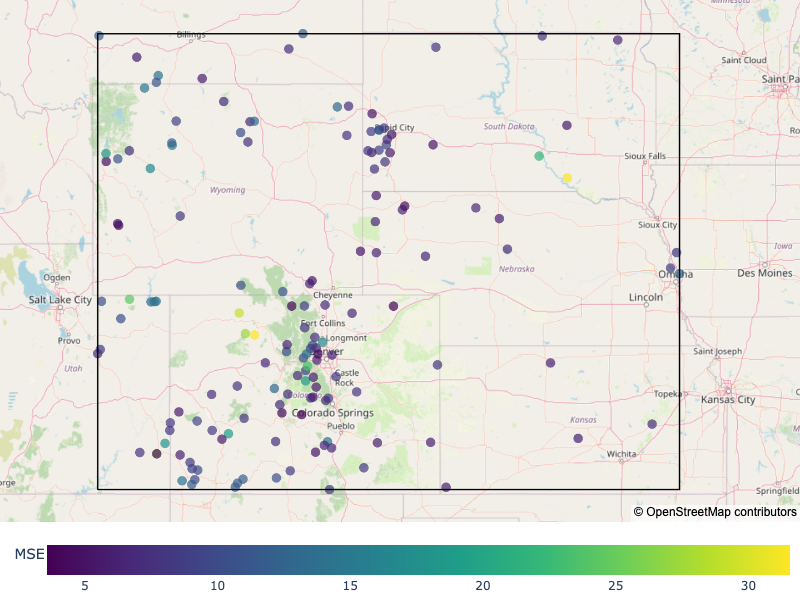
\includegraphics[width=12 cm]{Definitions/err_map}
\caption{Forecast Error by RAWS, averaged over all times and replications.}
\label{fig:err_map}
\end{figure}   


We evaluate the forecast error of the RNN and baseline models by the hour of the day (0-23 UTC). FMC varies throughout the day in a diurnal pattern, as shown in Figure~\ref{fig:ts}, so it is important to understand how this affects model accuracy. Figure~\ref{fig:err24} shows the forecast RMSE averaged across all locations, replications, and days of the year. All models show a relative peak in forecast RMSE from around 14:00 UTC, which corresponds to either 7:00am MST or 8:00am MDT. This is the time of the day when FMC tends to be the highest, since it is slightly after the lowest typical temperatures and highest typical RH of the day, and dew is often forming directly on the surface of the fuels at these times. In this study, the first hour of forecasting was fixed to be midnight 00:00 UTC, so we wish to quantify how the model error changes as the forecast is extended in time. The ODE+KF shows signs of recursive error accumulation, where the modeling error grows as the forecast continues to be extended in time. The XGBoost and climatology methods are not recursive, so there is no accumulation of forecast error. The RNN calculates loss by comparing the predicted FMC to a 48-hour stretch of observed FMC data, so the network is learning to minimize the error across this entire forecasting window. Thus, we do not observe recursive error accumulation in the RNN.

\begin{figure}[tbh]

\includegraphics[width=12 cm]{Definitions/err24}
\caption{Forecast error for RNN, ODE+KF, XGboost, and Climatology methods by hour of day, averaged over all locations, replications, and days of the year.}
\label{fig:err24}
\end{figure}   


%%%%%%%%%%%%%%%%%%%%%%%%%%%%%%%%%%%%%%%%%%
\section{Discussion}

% what was done here
In this study, we compared an RNN model of dead 10-h fuel moisture content with weather inputs from HRRR to several baseline methods. The accuracy of the models was compared when forecasting 48 hours into the future and at unobserved locations for all of 2024 in the Rocky Mountain region. The RNN was the most accurate model of FMC compared to the baseline methods, namely a physics-based model, a non-recursive ML model, and a climatology method, as shown in Section \ref{sec:results}. 

% comments on applicability - if definite, justify    
Forecasts from the RNN could be used within wildfire simulations that need to be run for multiple days. Additionally, forecasts from the RNN could be used to inform wildfire risk indices that provide warnings for areas prone to rapid wildfire spread.

% comments on ML techniques 
The RNN architecture used in this study was based on a restricted hyperparameter search scheme in the Rocky Mountain region. Spatial features were used as input to the RNN in this study, including elevation and latitude and longitude coordinates. In other geographic regions or on a national scale the choice of hyperparameters may be different. This will be evaluated in the future.

% comments on ML future
Future work will consider adding convolutional layers in combination with LSTM layers. Additionally, attention layers and transformers are alternatives to RNNs which have grown in popularity in recent years. We conducted minimal exploration with these methods and concluded that RNNs were preferable, but a full comparison of those model architectures should be considered in future work. 

% staking the ground
Future work will apply RNNs to other dead fuel classes, including 1-h and 100-h fuels. This modeling project only considered 10-h dead FMC since the vast majority of available data is for this fuel class. The RNN modeling approach in this paper could be adapted to model dead fuels of other sizes. Additionally, the RNN considered in this study will be tested using custom loss functions that attempt to account for the nonlinear relationship between FMC and wildfire rate of spread~\citep{Hirschi-2025-CLF}. Future research will examine additional predictors of FMC within the RNN, including satellite data products such as VIIRS reflectance bands and CYGNSS soil moisture. Finally, the RNN will be integrated into the WRF-SFIRE modeling project so that the FMC model can be tested on coupled wildfire simulations.

\vspace{6pt} 

%%%%%%%%%%%%%%%%%%%%%%%%%%%%%%%%%%%%%%%%%%
\authorcontributions{Jonathon Hirschi primary author, Jan Mandel initial RNN work and editing the manuscript, Angel FMC data collection and theoretical support, Kyle Hilburn general science support.}

\funding{The research presented in this paper was partially funded by NASA grants 80NSSC23K1118, 80NSSC22K1405, 80NSSC23K1344, and 80NSSC25K7276.
Computing resources were provided by the University of Colorado Denver supercomputing cluster Alderaan, partially funded by NSF Campus Cyberinfrastructure grant OAC-2019089.}

%% NOTE[At least we say: ``Data derived from public domain resources". Then decide if ``Data available in a publicly accessible repository" OR ``Data available on request due to restrictions" since large amount of compute is needed to host all the data for this project.]
\dataavailability{The code associated with this project was built in Python, and is publicly available at the GitHub repository \url{https://github.com/openwfm/ml_fmda}. This repository contains materials needed to reproduce the data set used in the analysis, the forecast accuracy metrics, talbes, and images. The data used in this project is derived from public domain resources, including the Amazon AWS data set of historical HRRR forecasts (\url{https://registry.opendata.aws/noaa-hrrr-pds/}) and the historical RAWS data from Synoptic, accessed through the software package SynopticPy (\url{https://github.com/blaylockbk/SynopticPy}). The data used in the project was collected, formatted, and stored using the University of Colorado Denver supercomputing cluster Alderaan. The exact data is available upon request due to privacy restrictions of the university computing system and the substantial storage space needed for this particular project.} 

\acknowledgments{A portion of this work used code generously provided by Brian Blaylock's Herbie Python packages Herbie (Version 2024.8.0) (\url{https://github.com/blaylockbk/SynopticPy}) and SynopticPy  (\url{https://github.com/blaylockbk/SynopticPy})}

\conflictsofinterest{The authors declare no conflicts of interest.} 

%%%%%%%%%%%%%%%%%%%%%%%%%%%%%%%%%%%%%%%%%%
%% Optional


\abbreviations{Abbreviations}{
The following abbreviations are used in this manuscript:
\\

\noindent 
\begin{tabular}{@{}ll}
FMC & Fuel Moisture Content\\
ML & Machine Learning\\
RNN & Recurrent neural network\\
LSTM & Long Short-term Memory\\
MSE & Mean squared error
\end{tabular}
}

%%%%%%%%%%%%%%%%%%%%%%%%%%%%%%%%%%%%%%%%%%
%% Appendix
\appendixtitles{yes} % Leave argument "no" if all appendix headings stay EMPTY (then no dot is printed after "Appendix A"). If the appendix sections contain a heading then change the argument to "yes".
\appendixstart
\appendix
\section[\appendixname~\thesection]{RNN Hyperparameter Tuning}
\label{sec:appendix_hyper}

Machine learning models have a set of fixed parameters that relate to model architecture or aspects of the fitting procedure, called ``hyperparameters''. These hyperparameters are fixed in the sense that they are not updated during the normal training process. Instead, they are ``tuned'' by repeatedly running the model with various sets of hyperparameters and comparing the resulting predictive accuracy. Neural networks have many hyperparameters, which can greatly affect the training process and final model accuracy. There are many methods for hyperparameter tuning. Grid search is a rigorous method of hyperparameter tuning where all possible combinations hyperparameters are compared within their given ranges. For neural networks, a full grid search usually results in a massive space of possible hyperparameter combinations that is not computationally feasible to search exhaustively. We utilized a restricted grid search, where a subset of the full number of hyperparameters was systematically explored, and other hyperparameters were fixed to theoretically or empirically justified defaults. 

Hyperparameter tuning was performed by training various model architectures on data from 2022 and evaluating forecast accuracy in 2023. Different model architectures and optimization parameters were evaluated on each of these forecast periods, and the overall model accuracy in terms of RMSE was averaged across all locations and times to compare models. 

The model architecture with the lowest forecast RMSE in 2023 was selected. The hyperparameters were fixed from this point on. The model was trained from scratch in 2023 and used to forecast the entire year of 2024. Randomization of the RAWS used in training versus testing ensures spatial independence. The temporal ordering of training and testing ensures causal realism, and ensures that the FMC observations from 2024 used to calculate the accuracy metrics presented in Section~\ref{sec:results} were not used in any way to conduct hyperparameter tuning.

We used a two-step hyperparameter tuning procedure. First, we tune the model architecture, including the type and number of hidden layers and the number of cell units per layer. The model architecture with the minimum average test RMSE from this step was used in the second stage of the hyperparameter tuning. In the second stage, hyperparameters related to optimization of trainable parameters were tuned, including batch size and learning rate. Using two stages in this way greatly reduces the number of possible model combinations and speeds up computation. 

For tuning the model architecture, we use the following constraints. We only consider LSTM and dense hidden layers. The LSTM layer(s) always precede the dense layers. We consider one, two, or three recurrent LSTM layers, and we consider zero, one, two, or three dense layers. For each layer, we consider a grid of numbers of units: 8, 16, 32, 128. Further, we impose a ``funnel'' like structure where the number of units always decreases or stays the same as you move across the layers from input to output. So, a layer with 64 units could feed into a 64, 32, or 16 unit layer, but a 16 unit layer can only feed into another 16 unit layer. For the optimization related parameters, we did a grid search for learning rate (0.05, 0.01, 0.005, 0.001, 0.0005, 0.0001) and batch size (16, 32, 64, 128). Candidate number of units and batch size are chosen to be powers of two, which in some computational contexts can lead to more efficient memory usage since binary computers usually have computational limits associated with powers of two.

Other hyperparameters were fixed across all models. These include, but are not limited to, the following. The list of predictors was fixed to be equilibrium moisture content, hourly rainfall, elevation, wind speed, downward shortwave radiation, and the longitude and latitude coordinates of the RAWS. The sequence length, or number of time steps, was set to 48 because the goal is to predict 48 hours into the future based on the forecast availability in the HRRR model. The activation functions were fixed to commonly accepted defaults for the layers. These are hyperbolic tangent (tanh) for LSTM activation, sigmoid for LSTM recurrent activation, and rectified linear (ReLu) for dense layers. A dropout rate of 15\% was used for dense layers and 20\% for the recurrent layers. Dropout is a common regularization technique in which in every training batch processed by the network, a random sample of given \% of the network weights is set to zero. The ``Adam'' optimizer was used in the training to minimize the loss function. Finally, we used early stopping with a patience of 5. This means that training is stopped if the accuracy on a validation set did not decrease for 5 epochs in a row. Using early stopping allows us to set the number of training epochs to a large number and avoid the need to tune this parameter. In practice, using 100 epochs with early stopping patience equal to 5 resulted in training where none of the iterations reached the maximum of 100, and training was typically halted after 5 to 10 epochs. 

%%%%%%%%%%%%%%%%%%%%%%%%%%%%%%%%%%%%%%%%%%

\begin{adjustwidth}{-\extralength}{0cm}
%} % If the paper is ``preprints'', please uncomment this parenthesis.
%\printendnotes[custom] % Un-comment to print a list of endnotes

\reftitle{References}

% Please provide either the correct journal abbreviation (e.g. according to the “List of Title Word Abbreviations” http://www.issn.org/services/online-services/access-to-the-ltwa/) or the full name of the journal.
% Citations and References in Supplementary files are permitted provided that they also appear in the reference list here. 

%=====================================
% References, variant A: external bibliography
%=====================================
\bibliography{references}



% If authors have biography, please use the format below
%\section*{Short Biography of Authors}
%\bio
%{\raisebox{-0.35cm}{\includegraphics[width=3.5cm,height=5.3cm,clip,keepaspectratio]{Definitions/author1.pdf}}}
%{\textbf{Firstname Lastname} Biography of first author}
%
%\bio
%{\raisebox{-0.35cm}{\includegraphics[width=3.5cm,height=5.3cm,clip,keepaspectratio]{Definitions/author2.jpg}}}
%{\textbf{Firstname Lastname} Biography of second author}

% For the MDPI journals use author-date citation, please follow the formatting guidelines on http://www.mdpi.com/authors/references
% To cite two works by the same author: \citeauthor{ref-journal-1a} (\citeyear{ref-journal-1a}, \citeyear{ref-journal-1b}). This produces: Whittaker (1967, 1975)
% To cite two works by the same author with specific pages: \citeauthor{ref-journal-3a} (\citeyear{ref-journal-3a}, p. 328; \citeyear{ref-journal-3b}, p.475). This produces: Wong (1999, p. 328; 2000, p. 475)

%%%%%%%%%%%%%%%%%%%%%%%%%%%%%%%%%%%%%%%%%%
%% for journal Sci
%\reviewreports{\\
%Reviewer 1 comments and authors’ response\\
%Reviewer 2 comments and authors’ response\\
%Reviewer 3 comments and authors’ response
%}
%%%%%%%%%%%%%%%%%%%%%%%%%%%%%%%%%%%%%%%%%%
\PublishersNote{}
%\isPreprints{}{% This command is only used for ``preprints''.
\end{adjustwidth}
%} % If the paper is ``preprints'', please uncomment this parenthesis.
\end{document}

